\section{\MakeUppercase{Theoretical Background}}
    \subsection{Introduction to Implicit Neural Networks (INNs)}
    \gls{inn} represent a class of deep learning models designed to learn an implicit function that maps input coordinates to output features. \gls{inn}s treat the weights of the network as data itself i.e. the data is represented within the weights of neural network. Unlike traditional neural networks that explicitly output values for each input in a dataset, \gls{inn}s define a continuous multidimensional function for the entire data space. This function can be evaluated at any point in its domain, making \gls{inn} especially suited for tasks involving high-dimensional data and requiring fine-grained control over outputs, such as in generating or reconstructing images, videos, and sounds. The basic concept of \gls{inn} can be visualized in the \autoref{fig:inr}
    \begin{figure}[H]
        \centering
        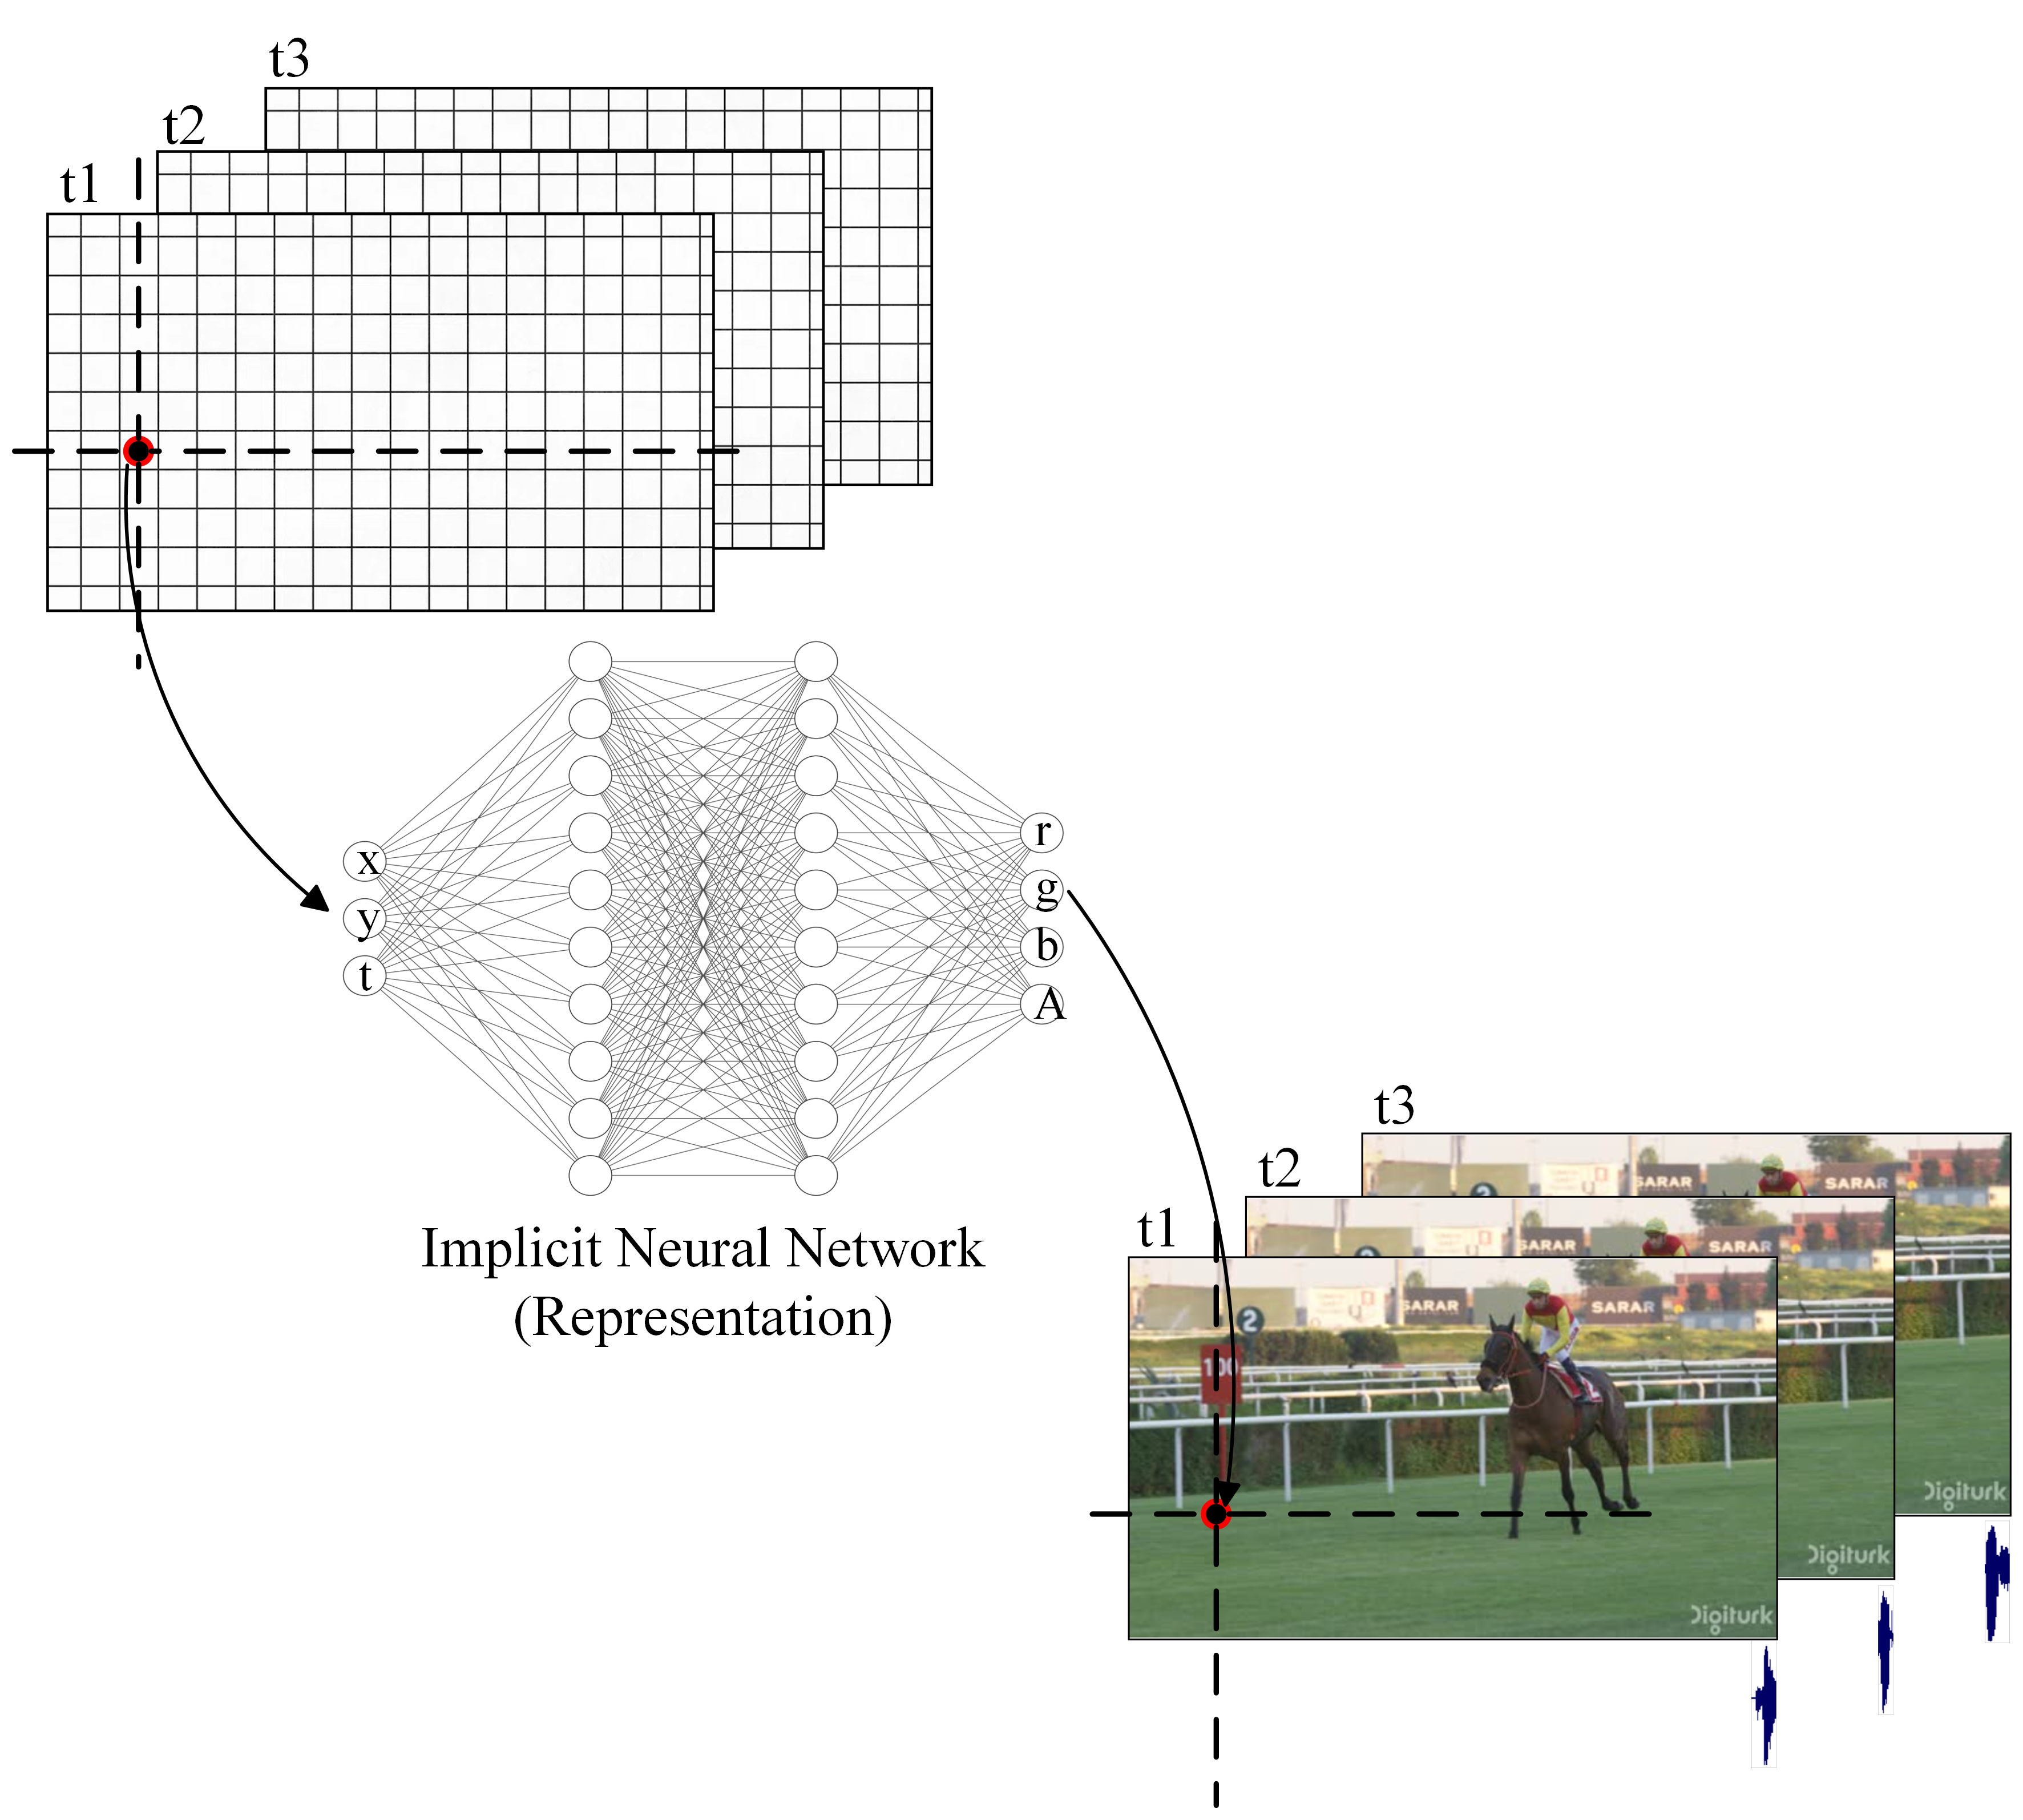
\includegraphics[height=0.45\textheight]{assets/INR.png}
        \caption{Representing Video in Neural Network}
        \label{fig:inr}
    \end{figure}
    \autoref{fig:inr} illustrates an Implicit Neural Representation (INR) where pixel coordinates $(x, y)$ and time index $t$ of video frames are fed into a neural network to output corresponding RGB values for visual data and amplitude for audio data. Sequential video frames $(t1, t2, t3)$ are divided into a grid of pixels. Each pixel's coordinates and time index are inputs to the network, which processes these inputs through several hidden layers. The network outputs the RGB values $(r, g, b)$ for each pixel's color and the amplitude $A$ for the associated audio. The outputs are then used to reconstruct the video frames and audio, demonstrating how the neural network encodes and decodes complex visual and audio information efficiently.
    \subsection{Fundamentals of INNs}
    \gls{inn} parameterize an unknown function \( f: \mathbb{R}^d \rightarrow \mathbb{R}^m \) where \( d \) and \( m \) represent the dimensions of the input and output spaces, respectively. This parameterization often involves a coordinate-based \gls{mlp} where the input coordinates are fed directly into the network, and the output is the function value at those coordinates. The network is trained using a loss function that minimizes the difference between the predicted and true function values over a set of sampled points.

    \subsection{Differences in Implicit Neural Network over Traditional Neural Network}

    The \autoref{fig:implicit-vs-traditional} provides a visual comparison between traditional neural networks and implicit neural networks like SIREN (Sinusoidal Representation Network). Traditional neural networks utilize a single set of shared weights and biases for all inputs, aiming to generalize across a dataset. This generalization allows the network to accurately classify or predict outcomes for new, unseen data based on its training. For instance, in the \autoref{fig:implicit-vs-traditional}, a traditional neural network trained on images of birds, reptiles, and mammals uses the same network architecture to classify any new image into these categories.

    In contrast, implicit neural networks represent each piece of media with its own unique neural network, characterized by distinct weights and biases. This approach fundamentally changes the way these networks operate. Overfitting, typically seen as a drawback in traditional neural networks, becomes a beneficial feature in implicit neural networks. Overfitting allows the network to memorize and accurately reproduce the intricate details and nuances of the specific piece of media it represents. For example, in the image, each silent video and audio clip has its own dedicated neural network that predicts frame-wise RGB values per pixel or time-wise amplitude values, respectively.

    The advantages of this approach are:

    \begin{itemize}
        \item \textbf{Detail Preservation:} The overfitting ensures that the network captures and reproduces fine-grained details of the media.
        \item \textbf{Per-Media Specialization:} Each piece of media is encoded into its unique network, allowing for highly specialized and optimized representations.
    \end{itemize}

    \begin{figure}[H]
        \centering
        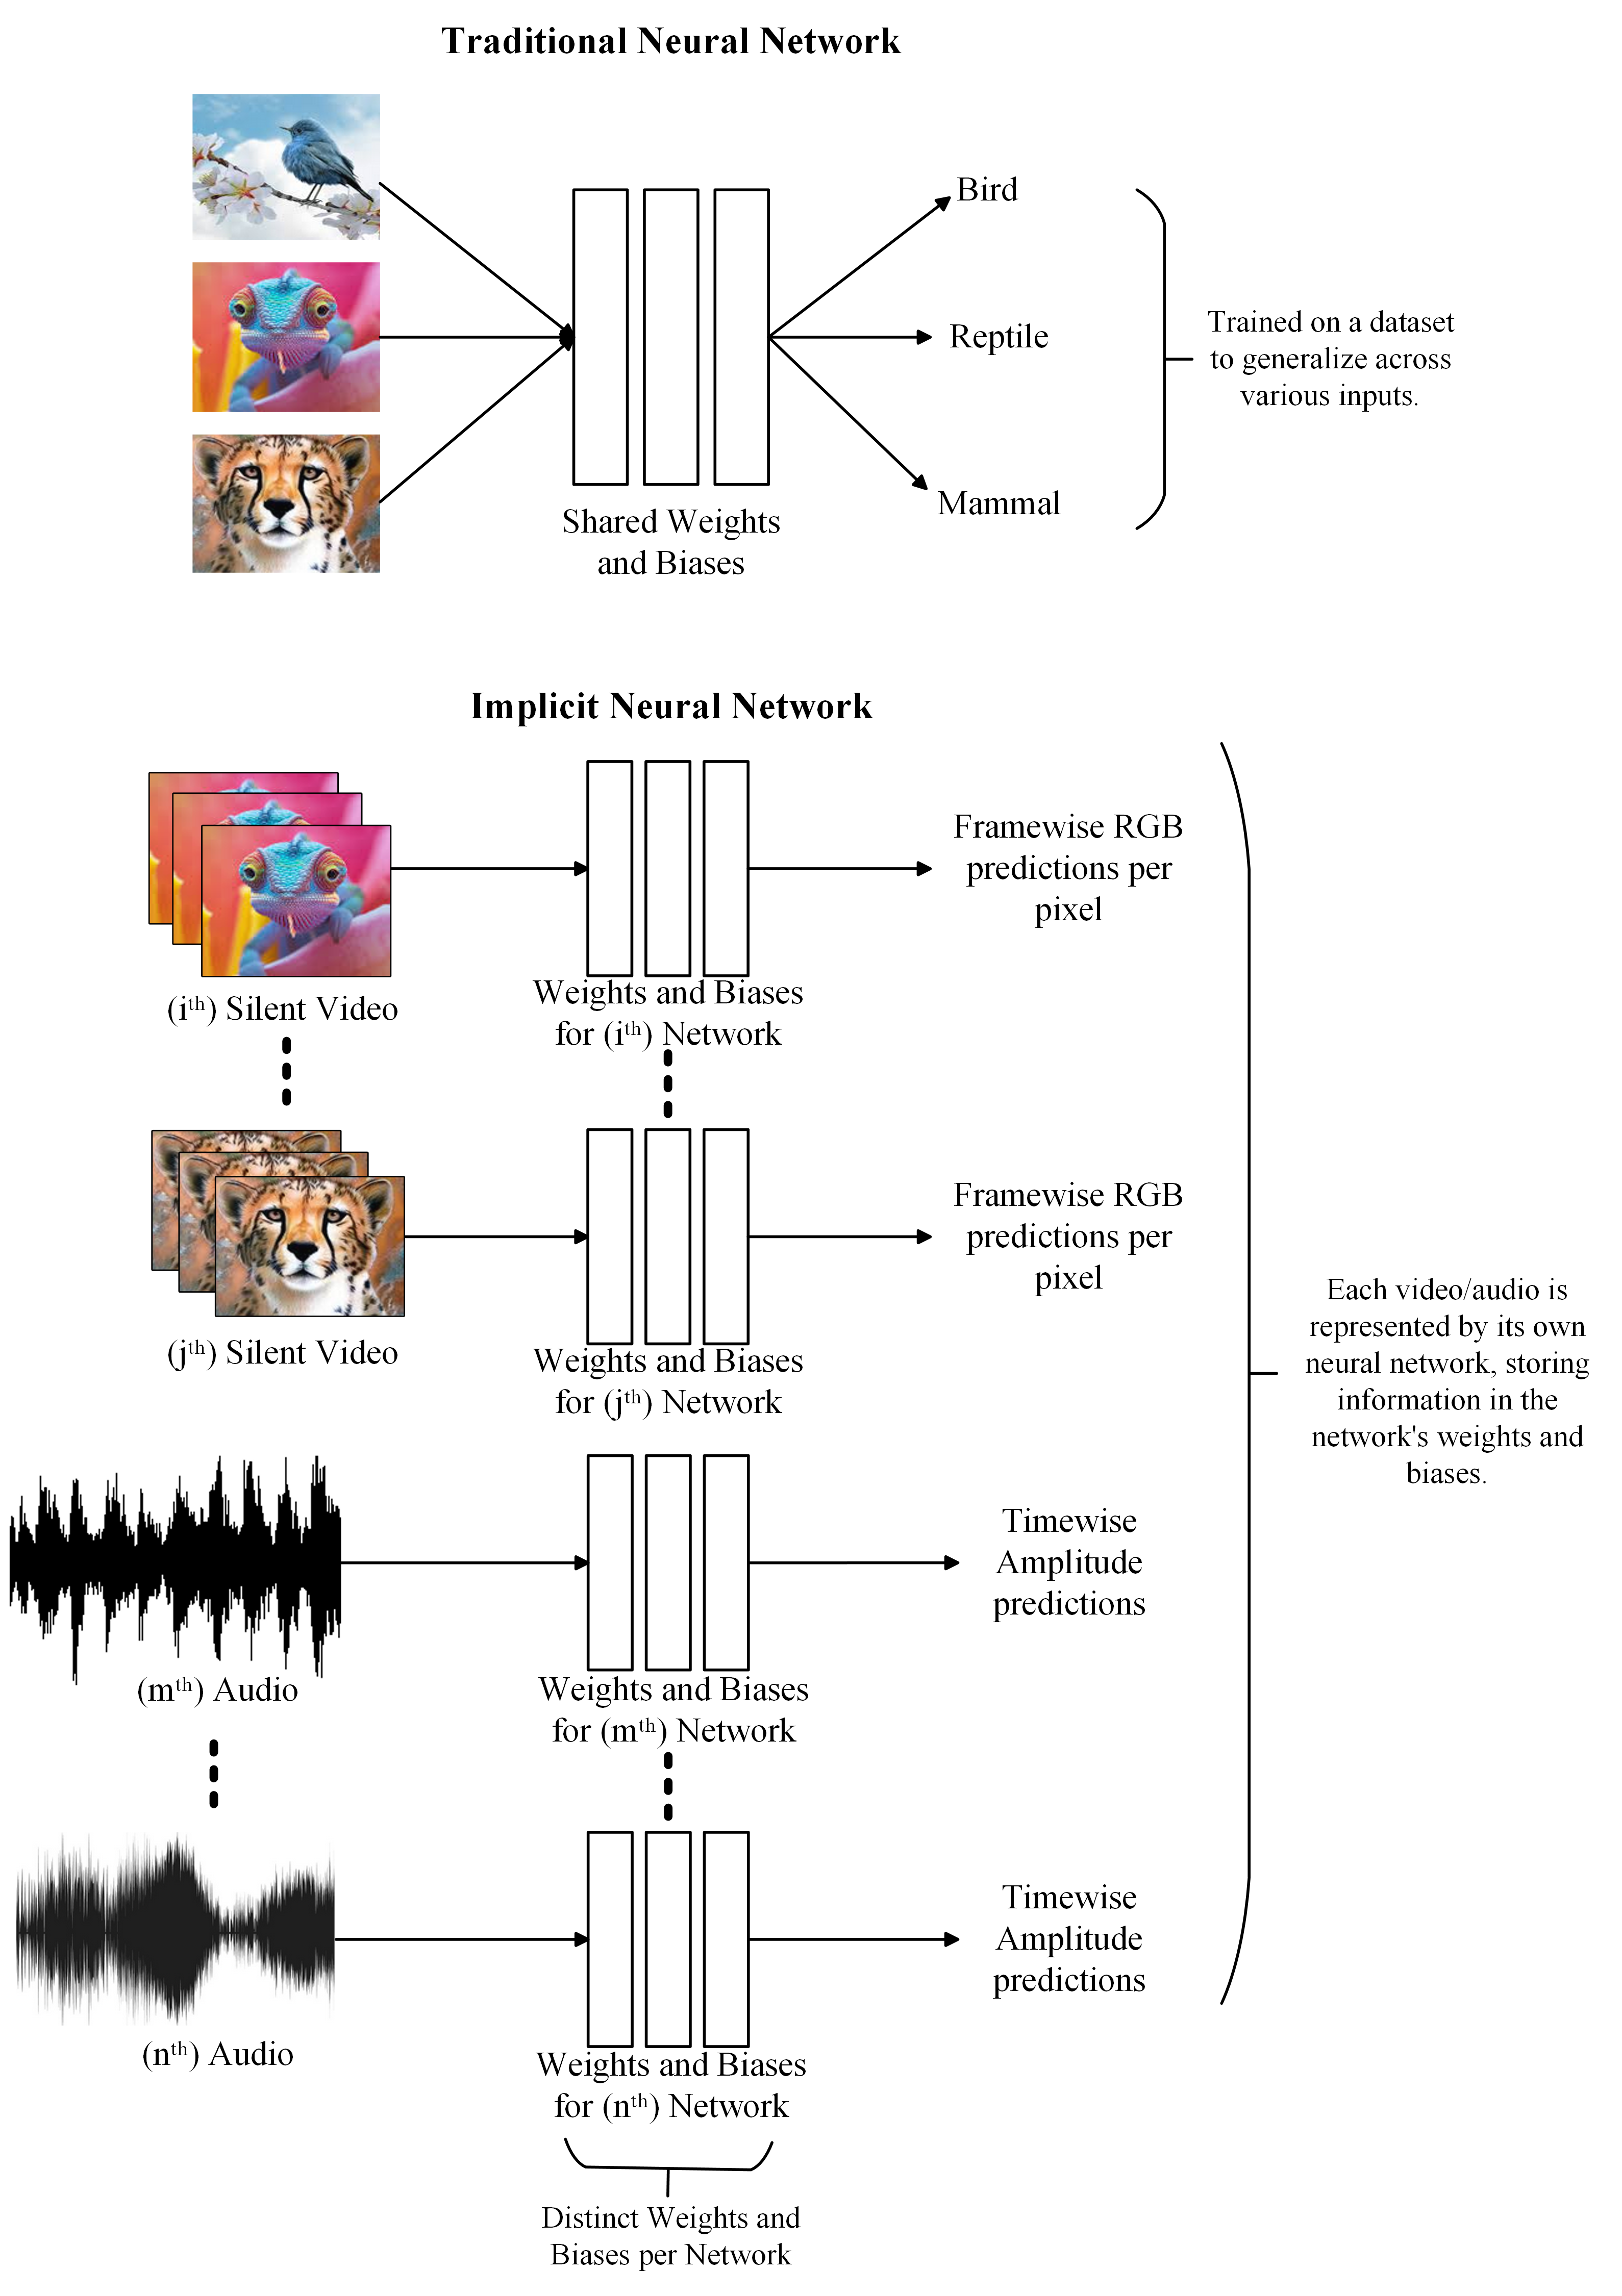
\includegraphics[width=0.95\linewidth]{assets/why overfitting.png}
        \caption{Implicit Neural Network vs Traditional Neural Network}
        \label{fig:implicit-vs-traditional}
    \end{figure}

    Thus implicit neural networks like \gls{siren} create unique networks for each media piece, leveraging overfitting to capture detailed representations. This allows implicit neural networks to store intricate details within their parameters, making overfitting a beneficial feature.
    
    
    \subsection{Significance of Sinusoidal Activations over Traditional Functions}

    The choice of activation functions in neural networks significantly influences their ability to model and process different types of data. The sine function is particularly suited for handling continuous inputs such as audio and video due to its inherent properties. Its smooth and periodic nature allows for efficient representation of continuous variations typical in audio waves or video frames. The smoothness of both the sine function and its derivative, a cosine wave, ensures that the gradients are well-defined across the entire function domain as shown in \autoref{fig:sinwave}. This characteristic is crucial during the neural network training process, which relies heavily on gradient-based optimization methods. The continuity and differentiability of the sine wave facilitate stable and effective weight updates, leading to reliable convergence in learning tasks.

    \begin{figure}[H]
        \centering
        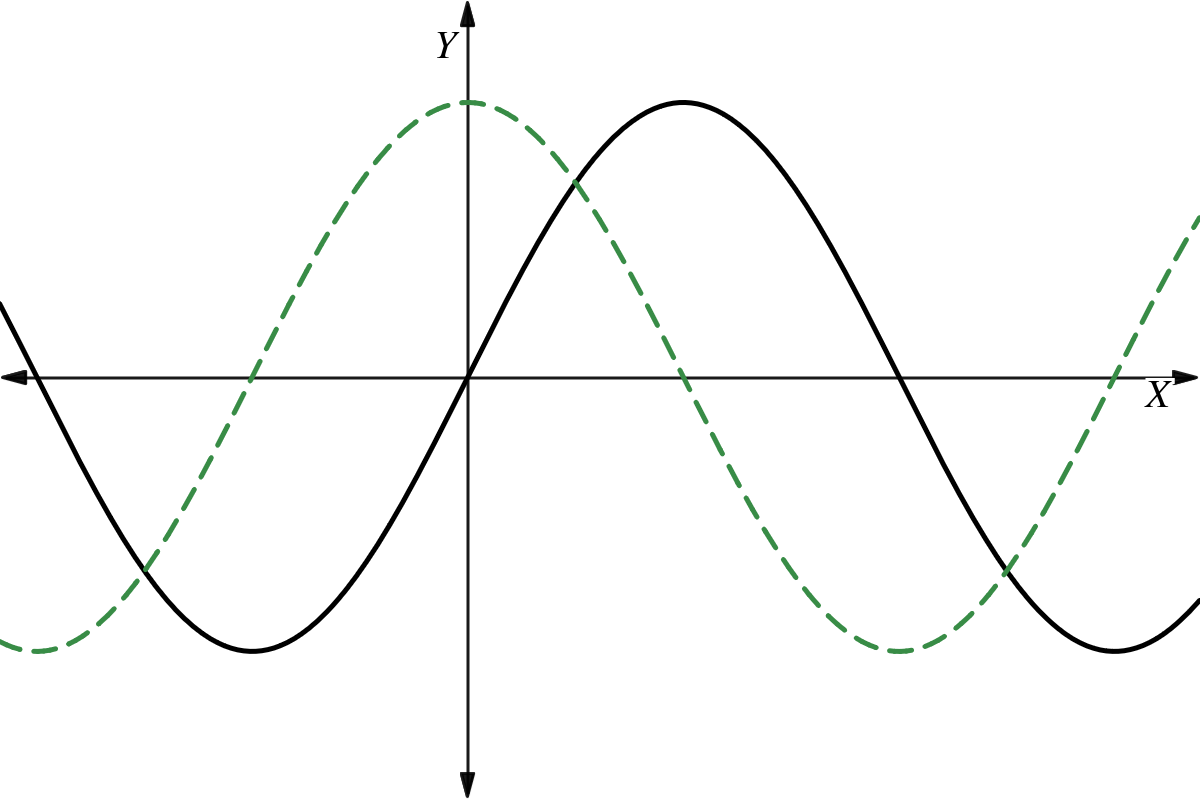
\includegraphics[height=0.25\textheight]{assets/sine-wave.png}
        \caption{Sine Wave and its Derivative}
        \label{fig:sinwave}
    \end{figure}

    In contrast, other waveforms like the triangular wave, although periodic, exhibit sharp transitions and corners at their peaks. The derivative of a triangular wave includes abrupt changes and discontinuities as we can see in \autoref{fig:triangular wave}, which can introduce complications in the learning process, particularly at points where the gradient becomes undefined. These discontinuities can potentially lead to instability in gradient calculations during backpropagation, adversely affecting the training efficiency and model performance. For neural networks involved in processing continuous data, such as in speech recognition or video processing, the sine function's ability to smoothly interpolate between values can capture complex, nuanced patterns more effectively. This smooth interpolation helps in better generalization and reduces the risk of overfitting to noisy variations, making the sine function a preferred choice for activation in networks dealing with continuous input signals.
    
    \begin{figure}[H]
        \centering
        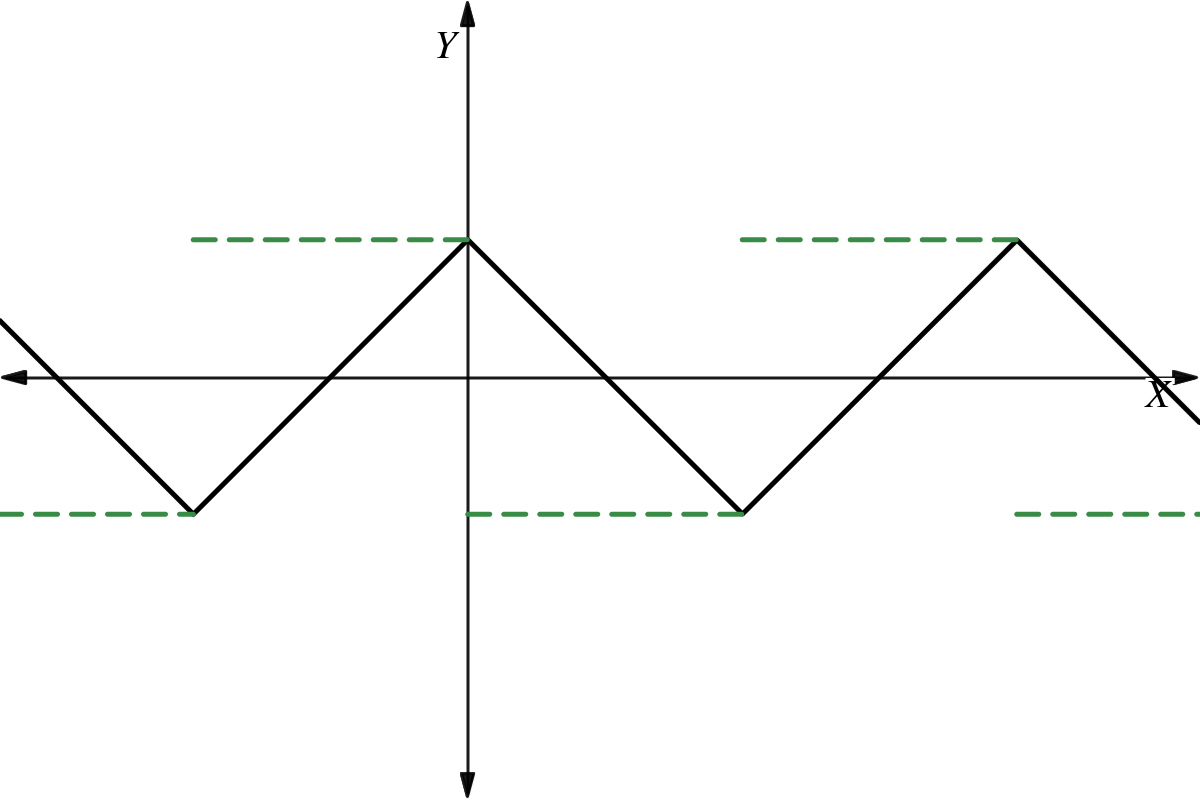
\includegraphics[height=0.25\textheight]{assets/triangular-wave.png}
        \caption{Triangular Wave and its Derivative}
        \label{fig:triangular wave}
    \end{figure}
    
    
    \begin{enumerate}[label=\textbf{\roman*.}]
        \item \textbf{Complex Signal Representation:} Sinusoidal activation functions enable neural networks to capture fine details and high-frequency components of signals more effectively. Traditional activation functions often struggle with this, leading to smoother, less detailed representations.
        \item \textbf{Smooth and Periodic Activation:} The smooth, continuous, and periodic nature of sinusoidal functions helps avoid issues like vanishing or exploding gradients, which are common with traditional activation functions, especially in deeper networks. This leads to more stable and efficient training dynamics.
        \item \textbf{Principled Initialization:} \gls{siren}s benefit from principled initialization scheme tailored for sinusoidal activations, ensuring that the network starts with a configuration that is conducive to learning complex patterns without the instability seen with other activation functions.
    \end{enumerate}
    
    \subsection{Transition to Sinusoidal Representation Networks (SIRENs)}
    Building on the concept of \gls{inn}, \gls{siren} introduce a critical innovation by employing sinusoidal activation functions in all layers of the network. The general form of a \gls{siren} layer is expressed as:
    \begin{equation}
        x_{i+1} = \sin(W_i x_i + b_i)
    \end{equation}
    
    where \( x_{i+1} \) is the output of the \(i\)-th layer, serving as the input to the next layer, \( \sin \) is the sinusoidal activation function applied to each layer, \( W_i \) is the weight matrix of the \(i\)-th layer, \( x_i \) is the input to the \(i\)-th layer, and \( b_i \) is the bias vector of the \(i\)-th layer.
    
    \subsection{Initialization Scheme for Sinusoidal Representation Networks (SIRENs)}
    Sinusoidal Representation Networks uses the sine function as an activation, which introduces sensitivity to input distributions due to its periodic nature. An effective initialization scheme is crucial to prevent the degradation of the network's performance with increasing depth. This report proposes a principled approach to initialization that preserves the distribution of activations across layers, ensuring that the output at initialization does not vary with the number of layers.
    \subsubsection{Steps Involved in Initialization}
    \begin{enumerate}[label=\textbf{\roman*.}]
        \item \textbf{Initial Input and Single Neuron Output}
        \begin{itemize}
            \item Uniformly Distributed Input: The input $x$ is drawn from a uniform distribution $U(-1, 1)$, representing normalized coordinates used in applications such as image processing.
            \item Output of a Single Sine Neuron: The output of a neuron using the sine activation function is given by:
               \begin{equation}
                  y = \sin(ax + b) 
               \end{equation} 
            where $a$ and $b$ are the frequency and phase parameters, respectively. For $a > \frac{\pi}{2}$, ensuring at least half a period of the sine function, the output distribution $y$ is arcsine distributed over $[-1, 1]$.
        \end{itemize}
        \item \textbf{Layer-wise Propagation}
        \begin{itemize}
            \item Weights and Biases: Weights $w$ are initialized uniformly within $U\left(-\frac{c}{\sqrt{n}}, \frac{c}{\sqrt{n}}\right)$ where, $c$ is a scaling factor and $n$ is the fan-in.
            \item Output of Deeper Layers: In subsequent layers, each input is arcsine distributed due to the previous layer's sine activation. The weighted sum $w^T x$ approaches a normal distribution as the number of inputs $n$ increases. Passing this sum through another sine function keeps the output arcsine distributed, preserving the distribution across layers.
        \end{itemize}
        \item \textbf{Special Handling in the First Layer} \\
          For the first layer, weights are adjusted by a factor $\omega_0$, set to 30. This adjustment ensures that the sine function: $\sin(\omega_0 \cdot Wx + b)$ spans multiple periods over the interval [-1, 1]. This extensive coverage is beneficial for handling the complex patterns and frequencies in video and audio data, enabling the network to capture a broad range of features initially.        
    \end{enumerate}


    \subsection{Siamese Siren}

    The Siamese Siren employs two neural networks with identical architectures but different weight initializations, referred to as the left and right Sirens. When an audio signal \( f \) is passed through these networks, they produce two slightly different outputs: \( f1 \) from the left Siren and \( f2 \) from the right Siren. These outputs, influenced by the slight variations in the networks, are then used to estimate and reduce noise.
    \begin{figure}[H]
        \centering
        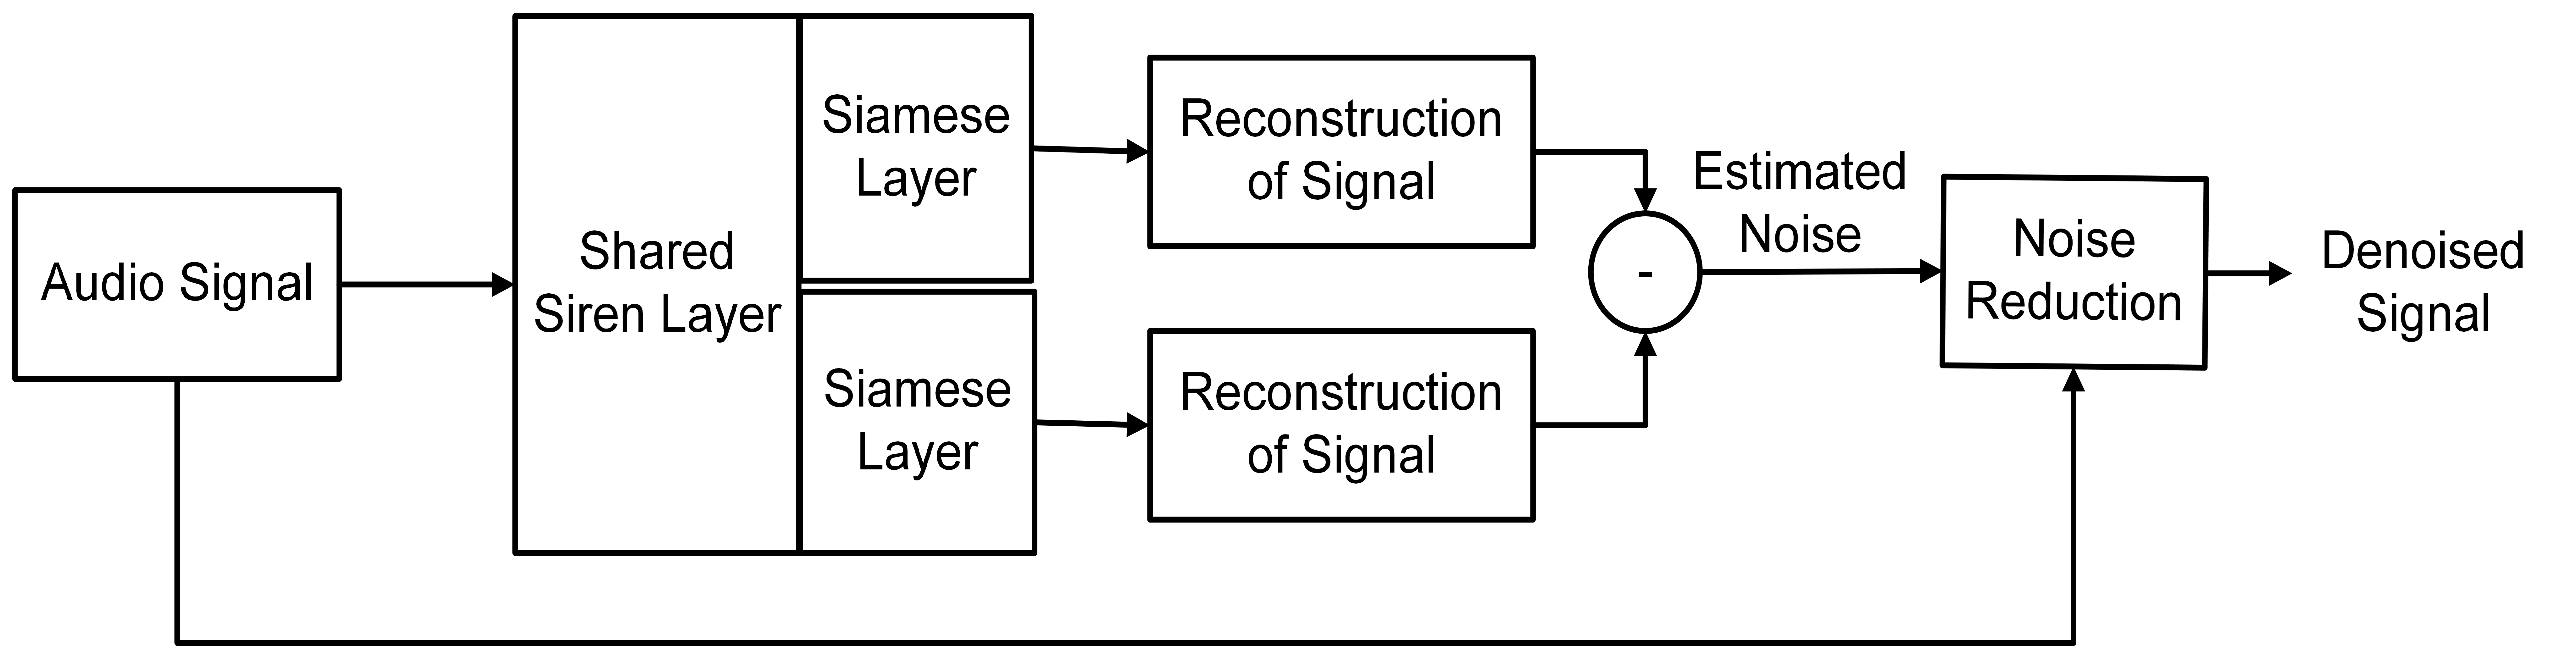
\includegraphics[width=\linewidth]{assets/Siamese_Siren_Block_Diagram.png}
        \caption{Siamese Siren Block Diagram}
        \label{fig:Siamese_Siren_Block_Diagram}
    \end{figure}

    \subsubsection{Noise Estimation in Siamese Siren}
    
    Siamese Siren estimates noise by calculating the difference between the outputs of the two networks:
    \begin{equation}
        \text{Noise} = f1 - f2
    \end{equation}
    where \( f1 \) is the inferenced audio from one network and \( f2 \) is the inferenced audio from the other network.
    
    \subsubsection{Noise Reduction Process}
    
    To reduce noise, the Siamese Siren leverages a noise reduction algorithm. This algorithm, often implemented using specialized noise reduction libraries, takes two inputs:
    \begin{enumerate}
        \item A noise estimation derived from the noisy audio.
        \item The noisy signal itself.
    \end{enumerate}

    \subsection{Knowledge Distillation for Model Compression}
    Knowledge distillation is a technique used in machine learning to transfer knowledge from a larger, more complex model (teacher) to a smaller, simpler model (student). This process aims to improve the efficiency and speed of the smaller model while maintaining or even enhancing its performance. One variant of knowledge distillation is \gls{rbkd}, which focuses on distilling knowledge related to the model's response or output behavior.

    The fundamental idea behind \gls{rbkd} is to train a student model to mimic not just the final predictions of the teacher model but also the intermediate responses or activations. This approach aims to capture the nuanced decision-making processes of the teacher model, enabling the student to generalize better and achieve comparable performance with fewer parameters.
    
    The main idea behind \gls{rbkd} revolves around the concept of feature representations and decision boundaries. By learning from the teacher model's response patterns, the student model can develop a deeper understanding of the underlying data distribution and make more informed predictions, especially in complex and high-dimensional input spaces.
    
    
    Soft Target Loss:
    The soft target loss remains the primary component in the distillation process. It compares the probabilities predicted by the student model to those of the teacher model:
    \begin{equation}
        L_{\text{soft}} = \frac{1}{N} \sum_{i=1}^{N} \left( S(x) - T(x)\right)^2
    \end{equation}
    
    where $L_{\text{soft}}$ is the soft target loss, $S(x)$ is the student model's output, and $T(x)$ is the teacher model's output for input $x$.

    Hard Target Loss:
    The hard target loss is an another component in response-based knowledge distillation. It compares the student model's predictions to the ground truth labels, ensuring that the student learns to represent the actual data accurately. The hard target loss is defined as:
    \begin{equation}
        L_{\text{hard}} = \frac{1}{N} \sum_{i=1}^{N} \left( S(x) - y\right)^2
    \end{equation}    
    
    where $L_{\text{hard}}$ is the soft target loss, $S(x)$ is the student model's output and $y$ is the ground truth label.

    The overall loss function simplifies to just the soft target loss without the response matching component:
    \begin{equation}
        L_{\text{total}} = \alpha L_{\text{soft}} + (1 - \alpha) L_{\text{hard}}
    \end{equation}

    where  $L_{\text{total}}$ is the total loss function, $\alpha$ is a hyperparameter controlling the importance of the soft target loss and hard target loss.
    
    In \autoref{fig:block-diagram-knowledge-distillation}, the teacher model is a SIREN (Sinusoidal Representation Networks) network pretrained on audio-visual data, while the student model is a shallower version designed to learn from the teacher's responses.
    
    The inputs to both models are in the form of (x, y, t), where (x, y) represent spatial coordinates in the video, and t represents time. The teacher model outputs four values: r, g, b (RGB values corresponding to (x, y, t)), and Amplitude (corresponding audio amplitude for the given (x, y, t)). Notably, the (x, y) coordinates are ignored in the context of audio amplitude.
    
    \begin{figure}[H]
        \centering
        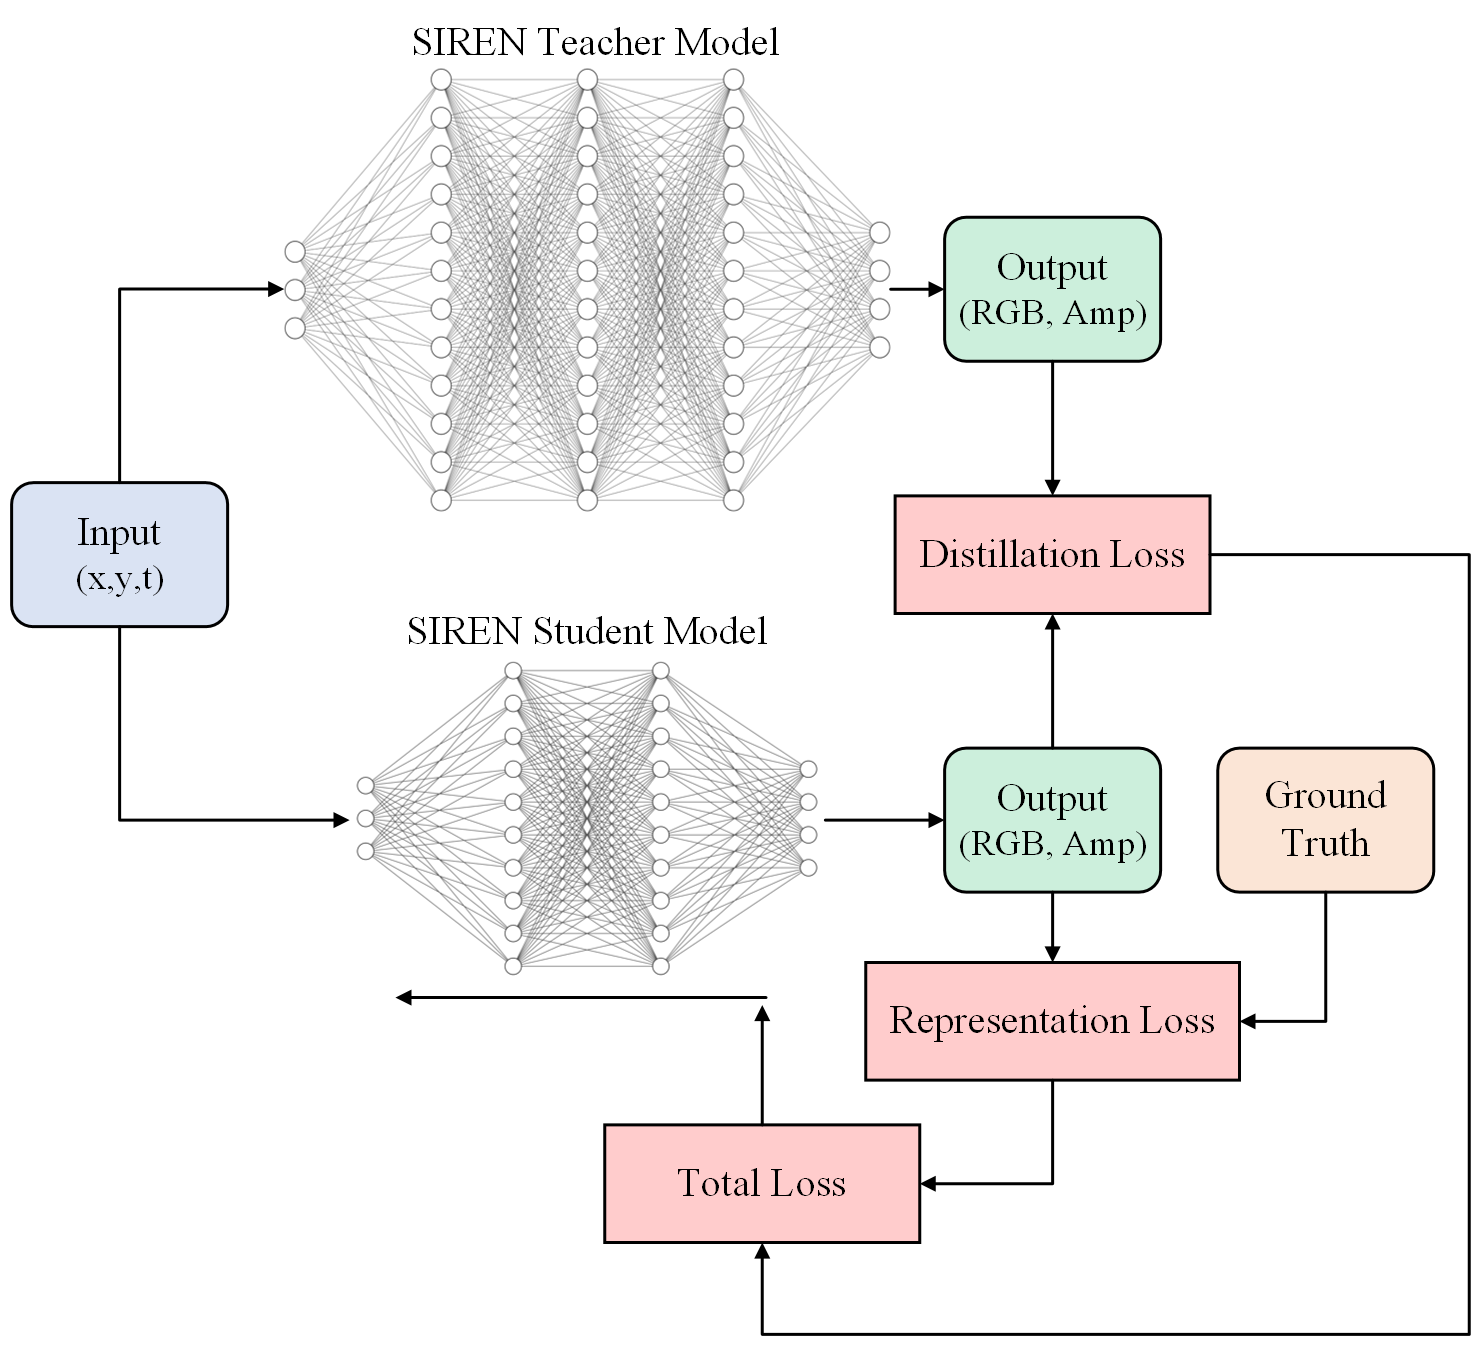
\includegraphics[width=0.95\linewidth]{assets/Knowledge Distillation.png}
        \caption{Block Diagram of Knowledge Distillation}
        \label{fig:block-diagram-knowledge-distillation}
    \end{figure}

    
    During response-based knowledge distillation, the student model's predictions are compared against the teacher model's predictions. This comparison helps calculate the distillation loss, which captures the discrepancy between the student's output and the teacher's output. Simultaneously, the ground truth provides the representation loss, measuring how well the student model represents the actual data.
    
    These two types of losses, distillation-loss and representation-loss, are weighted and combined to calculate the total loss. This total loss is then used for feedback and backpropagation during the training process, allowing the student model to gradually learn and mimic the behavior of the more complex teacher model.
    
    By using response-based knowledge distillation, the student model can benefit from the rich representations learned by the teacher model, even though it has a simpler architecture. This approach is particularly useful for tasks where computational resources or model complexity are constrained, yet high performance is desired.
      

    \subsection{Quantization}
    Quantization involves reducing the precision of the model's parameters, such as weights and biases, from floating-point to lower-bit representations, which decrease the model size.
    \begin{equation}
        w' = \text{round}\left(\frac{w}{s} + z \right)
    \end{equation}
    where, \( w \) is the original weight, \( s \) is a scaling factor, \( z \) is zero-point, and \( w' \) is the quantized weight.

    \begin{figure}[H]
            \centering
            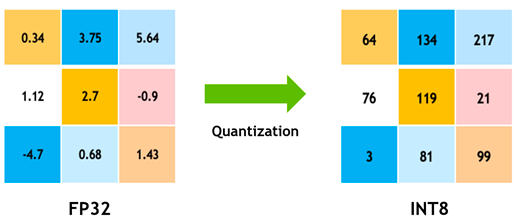
\includegraphics[width=\linewidth]{assets/quantization.png}
            \caption{Quantization}
            \label{fig:conceptual-quantization}
    \end{figure}
    In \autoref{fig:conceptual-quantization}, a sample 3x3 matrix of weights is taken. The weights are quantized to int 8, reducing the precision from 32-bit floating-point. This process reduces the model size and computational requirements, making it more efficient on resource-constrained devices.

    Since we will be using symmetric quantization for weights and biases of our model, we will discuss the symmetric quanzation below, however asymmetric quantization can also be done as shown in \autoref{app:quantization-manual-conversion}.
    \subsubsection{Symmetric Quantization} 
    \begin{figure}[H]
        \centering
        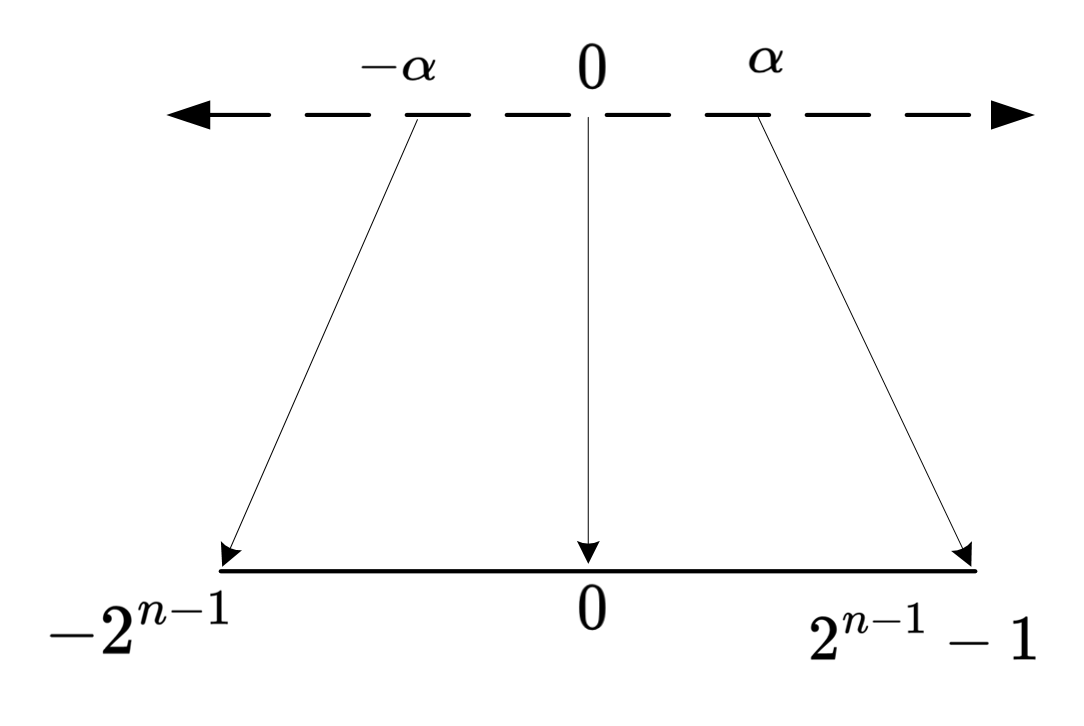
\includegraphics[width=0.7\linewidth]{assets/quantization/Symmetric_Qfigure.png}
        \caption{Symmetric Quantization}
        \label{fig:Symmetric_Qfigure}
    \end{figure}
    In symmetric quantization, the range of the values represented is symmetric around zero. This means the quantized values are distributed equally between positive and negative numbers.

    \textbf{Characteristics:}
    \begin{enumerate}
        \item Zero point is fixed at zero.
        \item Only scale factor is used to calculate quantized value.
    \end{enumerate}

    \subsection{Encoding}
    Encoding in the context of data compression refers to the process of converting raw data into a more compact representation, using techniques that minimize the amount of storage or transmission required. The goal of encoding is to reduce redundancy and increase efficiency, which can lead to significant reductions in the size of the data, making it easier to store and transfer.

    Two important methods for encoding data are Arithmetic Encoding and Range Encoding, which are widely used in various compression algorithms.

    \subsubsection{Arithmetic Encoding}
    Arithmetic Encoding is a form of entropy encoding that represents a message as a single number between 0 and 1. The key idea behind arithmetic encoding is to iteratively refine an interval to represent the entire message. Instead of encoding each symbol separately, arithmetic encoding encodes the entire message as a fraction in a range [0, 1].

    \begin{itemize}
        \item The process begins by initializing an interval [low, high], which initially spans the range [0, 1].
        \item For each symbol in the message, the interval is divided into subintervals based on the probabilities of the symbols. The interval is then updated based on the symbol's probability.
        \item The final encoded message is represented by a value within the resulting subinterval that corresponds to the entire message.
    \end{itemize}

    This method efficiently encodes data with different symbol frequencies and is highly effective in cases where symbols have different probabilities.

    \subsubsection{Range Encoding}

    \begin{figure}[H]
        \centering
        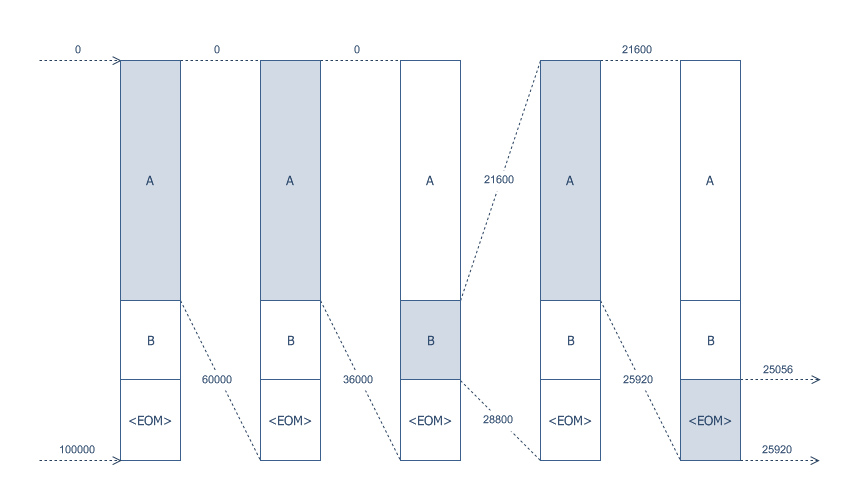
\includegraphics[width=0.95\linewidth]{assets/Range_encoding.jpg}
        \caption{Range Encoding}
        \label{fig:range_encoding}
    \end{figure}

    Range Encoding as shown in \autoref{fig:range_encoding} is similar to Arithmetic Encoding in that it also represents the entire message as a number within a range. However, Range Encoding uses a slightly different approach to dividing the range and updating it.

    \begin{itemize}
        \item Like arithmetic encoding, Range Encoding divides the range into subranges based on the probabilities of the symbols.
        \item However, Range Encoding works with fixed-size integers for each step, which makes it easier to implement and optimize.
        \item As each symbol is processed, the range is updated, and a final value within the range represents the compressed message.
    \end{itemize}

    While Range Encoding is simpler and faster than Arithmetic Encoding in practice, it can be less efficient when dealing with very large data sets or extremely small probabilities. Despite this, it remains popular in modern compression algorithms.

    % \subsection{Compression Algorithms}
    % Compression algorithms utilize encoding methods such as Arithmetic and Range Encoding to reduce the size of data. These algorithms are designed to identify patterns and redundancies in data, allowing them to replace these patterns with shorter representations, resulting in space savings.

    % \subsubsection{LZMA Algorithm}
    % The \gls{lzma} is a lossless data compression algorithm that employs both dictionary-based compression and range encoding. It is known for achieving very high compression ratios, making it a popular choice in formats such as 7z and xz.

    % LZMA uses a hybrid approach by combining two key techniques:
    % \begin{itemize}
    %     \item \textbf{Dictionary Compression:} \gls{lzma} maintains a sliding window (the dictionary), which stores previously seen data chunks. When encountering repeated sequences, \gls{lzma} replaces these sequences with references to their previous occurrences within the dictionary, allowing for significant compression.
    %     \item \textbf{Range Encoding:} To efficiently encode the references and symbols, \gls{lzma} uses Range Encoding. Range Encoding is applied to compress the frequency distribution of symbols and dictionary references. This step further reduces the size of the data by encoding the information in a compact form based on the likelihood of each symbol appearing.
    % \end{itemize}

    % The following is a simplified version of the \gls{lzma} algorithm:
    % \begin{enumerate}[label=\textbf{\roman*.}]
    %     \item \textbf{Initialization:}
    %     \begin{itemize}
    %         \item Build a dictionary of size \texttt{window\_size} to store previously encountered data.
    %         \item Set up a range encoder to start encoding the output.
    %     \end{itemize}
    %     \item \textbf{Input Processing:}
    %     \begin{itemize}
    %         \item Read a chunk of data from the input stream.
    %         \item For each symbol, check if it exists in the dictionary.
    %         \item If the symbol exists, output a reference to the dictionary.
    %         \item If the symbol doesn't exist, output the symbol itself and add it to the dictionary.
    %     \end{itemize}
    %     \item \textbf{Range Encoding:}
    %     \begin{itemize}
    %         \item For each reference or symbol, use range encoding to map it to a smaller numerical range.
    %         \item Adjust the range based on the probability distribution of the symbols and references.
    %     \end{itemize}
    %     \item \textbf{Finalize:}
    %     \begin{itemize}
    %         \item Complete the encoding and output the final compressed data stream.
    %     \end{itemize}
    % \end{enumerate}

    % This hybrid approach makes \gls{lzma} both highly efficient and scalable, able to achieve impressive compression ratios even on large datasets.

    % \subsubsection{xz}
    % The xz compression format implements the \gls{lzma} algorithm, making use of the hybrid dictionary and range encoding approach to achieve high compression efficiency. xz is a popular compression utility used in Linux distributions and other environments that require strong compression performance.

    % xz specifically implements \gls{lzma}2, a variant of the \gls{lzma} algorithm, which provides enhanced parallelism, allowing for better use of multi-core processors and increased compression speed without sacrificing compression ratio.

    % Key characteristics of xz's implementation of \gls{lzma} are:

    % \begin{itemize}
    %     \item \textbf{Dictionary Management:} Similar to \gls{lzma}, xz uses a dictionary-based approach where repeated strings in the input data are replaced by references to previous occurrences. This dictionary can be large and is critical for achieving high compression ratios.
    %     \item \textbf{Parallelization:} xz introduces the \gls{lzma}2 format, which divides the compression task into blocks. This allows multiple blocks to be compressed in parallel, making xz suitable for modern hardware with multiple processors or cores.
    %     \item \textbf{Range Encoding:} xz uses Range Encoding, just like \gls{lzma}, to encode the dictionary references and symbols, optimizing the final compressed output.
    % \end{itemize}

    % The xz format is widely used for distributing software packages, particularly in environments where high compression ratios are important. By implementing \gls{lzma}2 with range encoding and dictionary compression, xz can achieve impressive compression ratios while maintaining high performance.
    \subsubsection{LZMA2 Algorithm}
    The \gls{lzma}2 algorithm is an enhanced successor to the original \gls{lzma} (Lempel-Ziv-Markov chain Algorithm). While retaining the core principles of \gls{lzma}, \gls{lzma}2 addresses several limitations and introduces critical improvements, particularly for modern hardware and large datasets. It is the algorithm used in the xz compression format and is optimized for both compression ratio and performance.
    
    \gls{lzma}2 combines dictionary-based compression with range encoding, similar to \gls{lzma}, but adds the following key features:
    \begin{itemize}
        \item \textbf{Block-Based Processing:} \gls{lzma}2 divides input data into independently compressible blocks. This enables parallel processing, allowing multi-core systems to compress or decompress multiple blocks simultaneously, significantly improving speed.
        \item \textbf{Adaptive Dictionary Management:} Unlike \gls{lzma}, which uses a single continuous dictionary, \gls{lzma}2 resets or updates the dictionary between blocks. This prevents the dictionary from becoming overly large or inefficient when processing heterogeneous data.
        \item \textbf{Handling of Incompressible Data:} \gls{lzma}2 detects incompressible regions and stores them uncompressed, avoiding unnecessary computational overhead. This contrasts with \gls{lzma}, which would still attempt to compress such data.
        \item \textbf{Streamable Processing:} \gls{lzma}2 supports seamless compression of continuous data streams without requiring full data availability upfront, making it suitable for real-time applications.
    \end{itemize}
    
    The algorithm operates as follows:
    \begin{enumerate}[label=\textbf{\roman*.}]
        \item \textbf{Initialization:}
        \begin{itemize}
            \item Configure block size and thread count for parallel processing.
            \item Initialize a range encoder and allocate dictionaries for each block.
        \end{itemize}
        \item \textbf{Block Processing:}
        \begin{itemize}
            \item Split the input data into blocks (if parallelization is enabled).
            \item For each block, apply dictionary compression:
            \begin{itemize}
                \item Replace repeated sequences with references to the block-specific dictionary.
                \item Add new symbols to the dictionary dynamically.
            \end{itemize}
        \end{itemize}
        \item \textbf{Range Encoding:}
        \begin{itemize}
            \item Encode the compressed blocks using range encoding, adjusting probabilities based on symbol frequency.
            \item For incompressible blocks, encode raw data directly.
        \end{itemize}
        \item \textbf{Output Finalization:}
        \begin{itemize}
            \item Combine encoded blocks into a single compressed stream.
            \item Add metadata (e.g., block boundaries, dictionary reset flags).
        \end{itemize}
    \end{enumerate}
    
    Compared to \gls{lzma}, \gls{lzma}2 provides:
    \begin{itemize}
        \item \textbf{Scalability:} Efficient utilization of multi-core CPUs via parallel block compression.
        \item \textbf{Flexibility:} Adaptive handling of mixed compressible/incompressible data.
        \item \textbf{Resource Efficiency:} Reduced memory overhead through dictionary resets.
    \end{itemize}
    
    \subsubsection{xz}
    The xz compression format is the primary implementation of \gls{lzma}2. It leverages the algorithm's block-based design and parallelization capabilities to achieve high compression ratios while maintaining competitive speeds on modern hardware. xz is widely adopted in Linux distributions for software distribution and archival purposes.
    
    Key features of xz include:
    \begin{itemize}
        \item \textbf{Multi-Threaded Compression:} By default, xz uses \gls{lzma}2's block partitioning to distribute workloads across CPU cores.
        \item \textbf{Configurable Block Sizes:} Users can optimize for speed or ratio by adjusting block sizes.
        \item \textbf{Backward Compatibility:} xz supports legacy \gls{lzma} for decompression, ensuring interoperability with older systems.
    \end{itemize}
    
    xz's integration of \gls{lzma}2 makes it a versatile tool for scenarios demanding both high compression efficiency and performance, such as large-scale data backups or software package distribution.
    \subsection{MPEG Audio Layer 3}
    MPEG Audio Layer 3, commonly known as MP3, is a widely used audio compression standard that reduces file size while preserving perceptual audio quality. The encoding process involves several stages that progressively transform and compress the digital audio signal into a highly efficient format.
    
    \subsubsection{MPEG Audio Layer 3 Encoder}
        \begin{figure}[H]
            \centering
            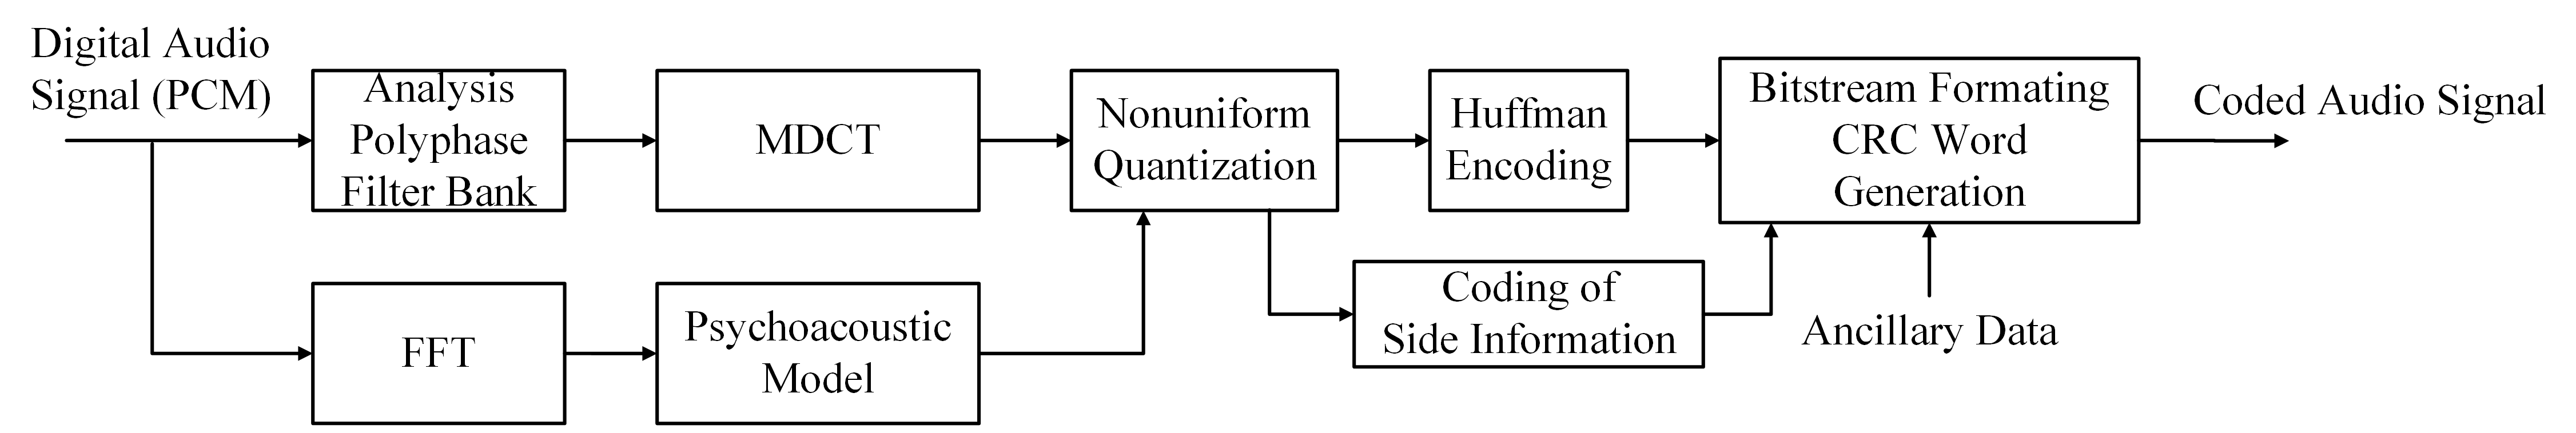
\includegraphics[width=0.95\linewidth]{assets/mp3_encoder.png}
            \caption{MPEG Audio Layer 3 Encoder}
            \label{fig:mp3_encoder}
        \end{figure}

        \begin{enumerate}[label=\textbf{\roman*.}]
            \item \textbf{Digital Audio Signal (PCM):}  
            \gls{pcm} represents the raw, uncompressed digital audio signal. It consists of sampled values of the original sound waveform, typically represented as 16-bit signed integers per sample. The input to the MP3 encoder is PCM audio, commonly sampled at rates like 44.1 kHz (CD quality) or 48 kHz.
        
            \item \textbf{Analysis Polyphase Filter Bank:}  
            This stage splits the audio signal into sub-bands or frequency bands using a polyphase filter bank. Dividing the signal into smaller frequency channels simplifies further processing and enables selective compression.
        
            \item \textbf{FFT (Fast Fourier Transform):}  
            The \gls{fft} converts the time-domain audio signal into the frequency domain. This transformation identifies the energy in different frequency components (sine waves) of the audio, providing insight into the spectral content.
        
            \item \textbf{Psychoacoustic Model:}  
            The psychoacoustic model applies principles of human hearing to discard inaudible data.
            \begin{itemize}
                \item Frequencies above 20 kHz or below the threshold of hearing are removed.
                \item Masking effects eliminate inaudible sounds masked by louder frequencies.
                \item Loudness analysis determines the importance of each frequency band, prioritizing perceptually significant data.
            \end{itemize}
        
            \item \textbf{MDCT (Modified Discrete Cosine Transform):}  
            \gls{mdct} further processes the frequency data by converting overlapping audio blocks into the frequency domain. It reduces blocking artifacts and provides better time-frequency resolution. This step ensures accurate reconstruction during decoding.
        
            \item \textbf{Nonuniform Quantization:}  
            The MDCT coefficients are quantized to compress the audio further:
            \begin{itemize}
                \item Frequencies less perceptible to the human ear are quantized with less precision.
                \item This step introduces bit-rate control, selectively reducing precision to minimize file size while maintaining quality.
            \end{itemize}
        
            \item \textbf{Huffman Encoding:}  
            A lossless compression technique is applied to the quantized data. Huffman encoding assigns shorter codes to frequently occurring values, optimizing the overall file size.
        
            \item \textbf{Bitstream Formatting and CRC Word Generation:}  
            The encoded audio data is organized into a structured bitstream. \gls{crc} data is added to verify data integrity during transmission.
        
            \item \textbf{Coding of Side Information:}  
            Side information includes metadata required for decoding:
            \begin{itemize}
                \item Sampling rate
                \item Bitrate
                \item Frame length
                \item Quantization details
            \end{itemize}
            This ensures accurate reconstruction of the audio.
        
            \item \textbf{Ancillary Data:}  
            Optional ancillary data, such as metadata (ID3 tags), album art, or custom data, can be embedded in the MP3 file. Although not required for decoding, it adds extended functionality.
        \end{enumerate}

        \subsubsection{MPEG Audio Layer 3 Decoder}

        \begin{figure}[H]
            \centering
            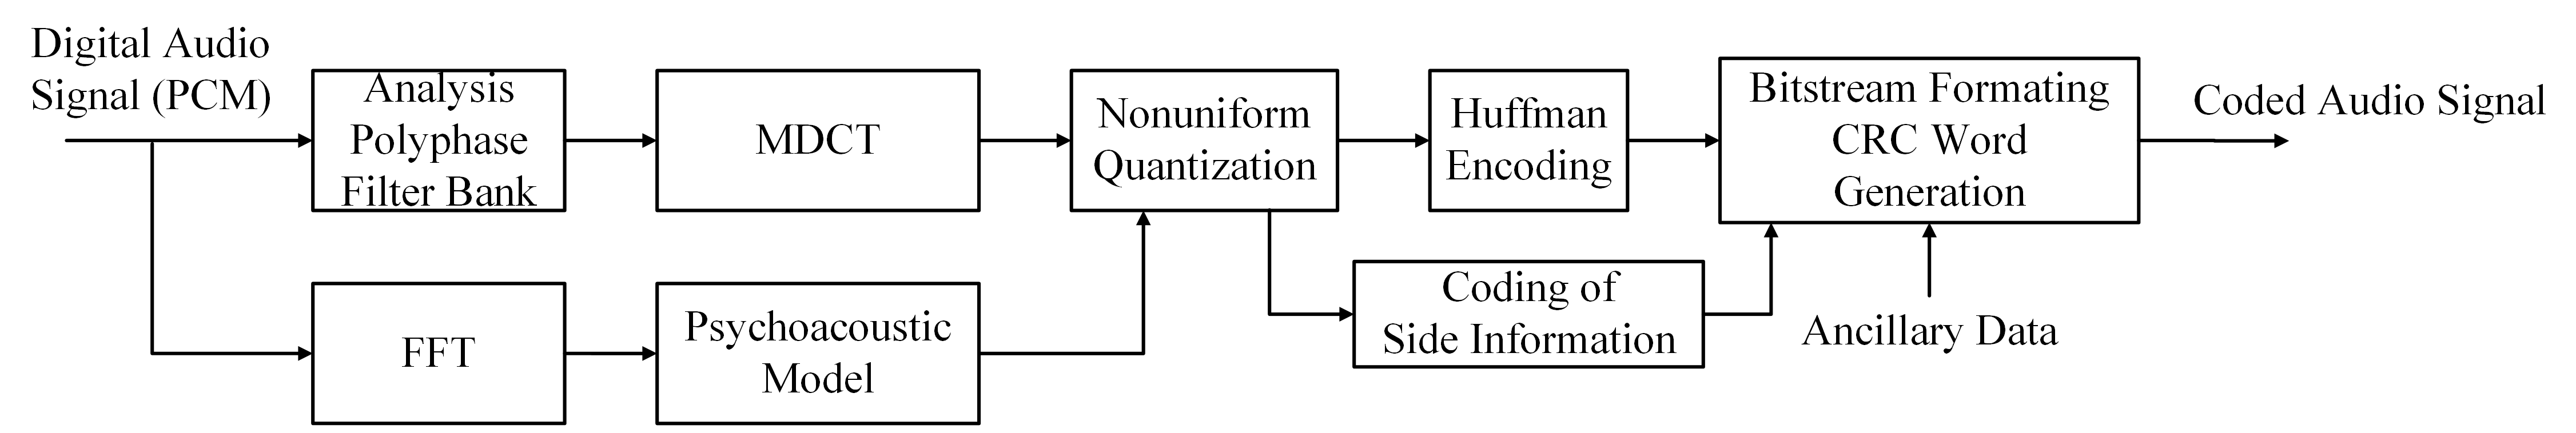
\includegraphics[width=0.95\linewidth]{assets/mp3_encoder.png}
            \caption{MPEG Audio Layer 3 Decoder}
            \label{fig:mp3_decoder}
        \end{figure}
        
        \begin{enumerate}[label=\textbf{\roman*.}]
            \item \textbf{Bitstream:}  
            The bitstream is the compressed MP3 file produced during encoding. It contains the encoded audio data along with side information necessary for decoding.
        
            \item \textbf{Synchronization and Error Checking:}  
            This block resolves synchronization issues in the bitstream and verifies its integrity using techniques like CRC (Cyclic Redundancy Check).
        
            \item \textbf{Huffman Decoding:}  
            This step reverses the Huffman encoding applied during compression, recovering the quantized audio data.
        
            \item \textbf{Scalefactor Decoding:}  
            The scalefactor values embedded in the bitstream are decoded. These values are crucial for restoring the magnitude of the frequency-domain coefficients.
        
            \item \textbf{Descaling:}  
            The quantized values are rescaled to their proper range to ensure accurate reconstruction of the audio data.
        
            \item \textbf{Reordering:}  
            The data reordered during encoding for compression efficiency is restored to its original order.
        
            \item \textbf{Joint Stereo Decoding:}  
            If joint stereo techniques were used in encoding, the stereo channels are reconstructed. This step restores the correlation between the left and right channels.
        
            \item \textbf{Alias Reduction:}  
            Alias reduction eliminates aliasing artifacts caused during the encoding process, ensuring clean audio output.
        
            \item \textbf{IMDCT (Inverse Modified Discrete Cosine Transform):}  
            The \gls{imdct} step reverses the \gls{mdct} transformation applied during encoding, converting frequency-domain data back into the time domain.
        
            \item \textbf{Frequency Inversion:}  
            Any frequency inversion applied during encoding is reversed in this step.
        
            \item \textbf{Synthesis Polyphase Filter Bank:}  
            The Synthesis Polyphase Filter Bank reconstructs the original time-domain signal from the time-frequency data. It operates as the inverse of the Analysis Polyphase Filter Bank used during encoding.
        
            \item \textbf{PCM Output:}  
            The final output is in Pulse Code Modulation \gls{pcm} format, an uncompressed audio representation ready for playback. Separate left and right channels are produced for stereo audio.
        \end{enumerate}
        
    \subsection{Advanced Video Codec (AVC) }
        \begin{figure}[H]
        \centering
        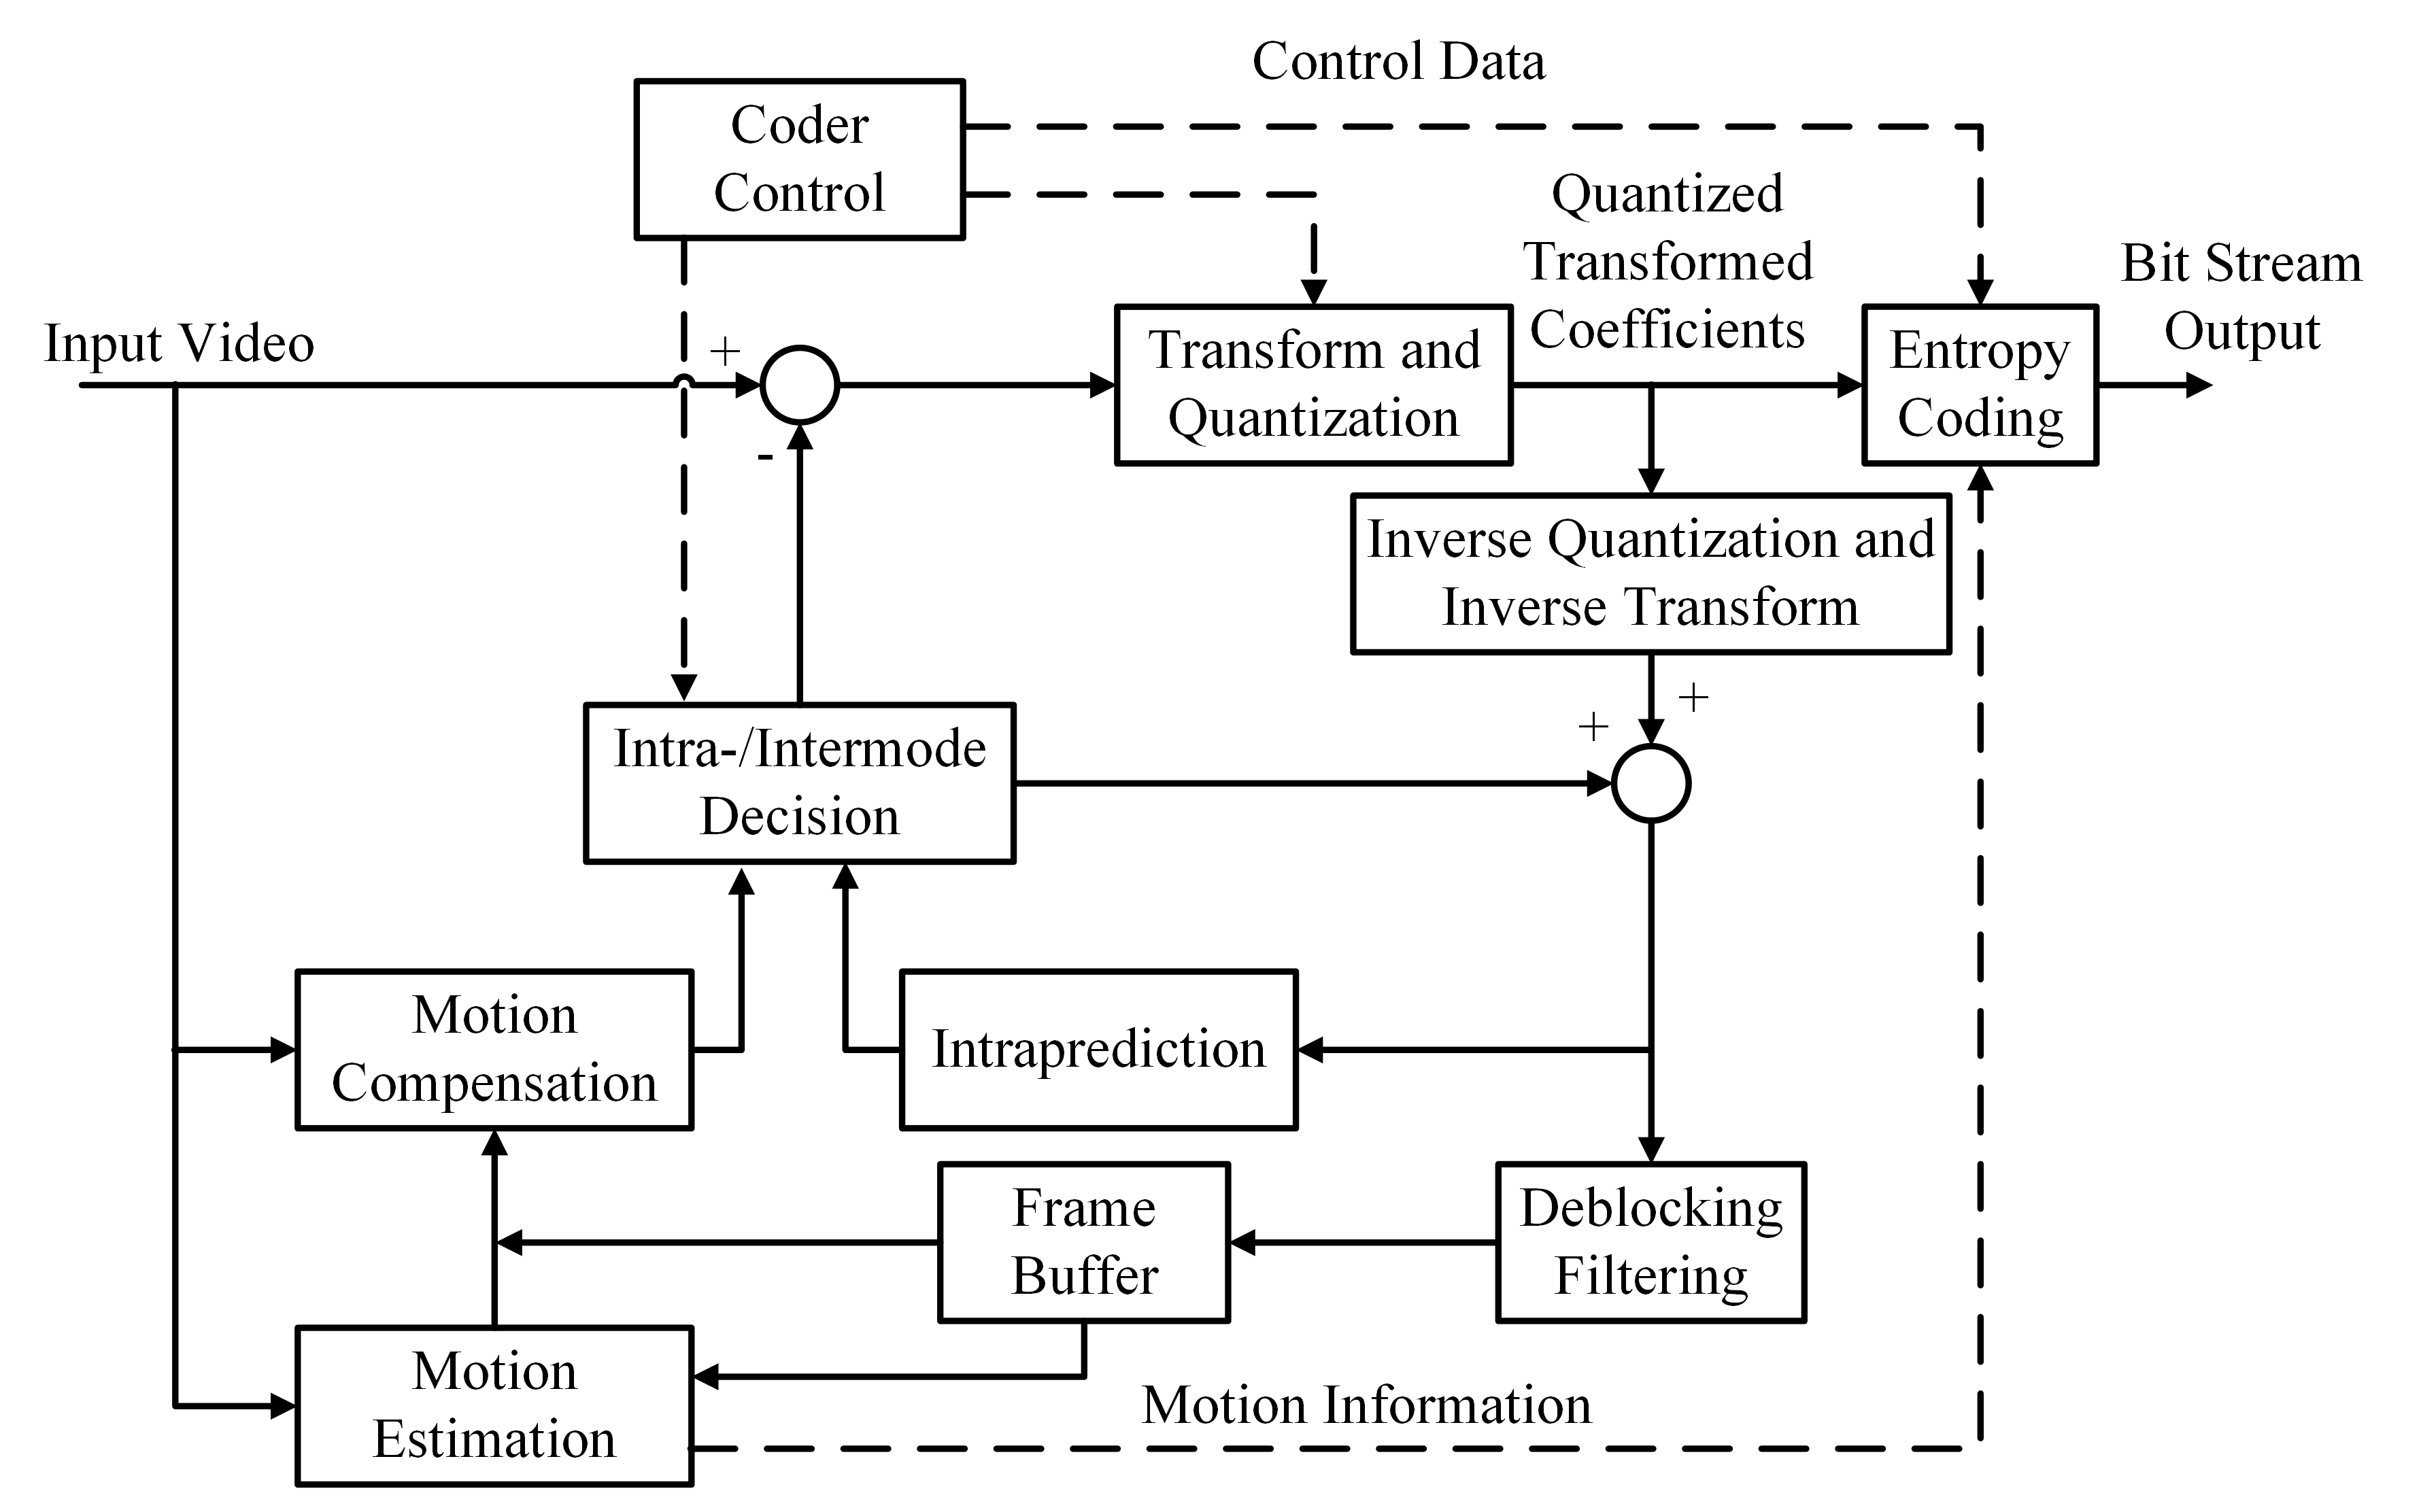
\includegraphics[width=0.95\linewidth]{assets/h264_blockdiagram.png}
        \caption{Block Diagram of Advanced Video Codec}
        \label{fig:avc}
    \end{figure}

    \autoref{fig:avc} outlines the encoding process for the Advanced Video Codec. The process involves a series of steps, starting with the input video and proceeding through various prediction, transformation, and compression techniques to produce a highly efficient encoded bitstream. 

    \begin{enumerate}[label=\textbf{\roman*.}]
        \item \textbf{Input Video:}  
        The process begins with an input video consisting of a sequence of frames, each composed of three components: luminance (Y) and chrominance (Cb and Cr). The luminance provides brightness information, while chrominance adds color details. Frames are divided into macroblocks of $16 \times 16$ pixels for Y and $8 \times 8$ pixels for Cb and Cr.
    
        \item \textbf{Intra-/Intermode Decision:}  
        This step determines how each macroblock will be encoded.
        \begin{itemize}
            \item \textbf{Intra-mode:} Macroblocks are predicted based on previously encoded blocks within the same frame. This mode is effective for spatial redundancy.
            \item \textbf{Inter-mode:} Macroblocks are predicted using reference frames from the past or future. This mode is effective for temporal redundancy.
        \end{itemize}
    
        \item \textbf{Motion Estimation:}  
        When inter-mode is selected, motion estimation determines object movement relative to reference frames.
        \begin{itemize}
            \item Macroblocks can be divided into smaller partitions (e.g., $16 \times 16$, $8 \times 8$, $4 \times 4$).
            \item Motion vectors with sub-pixel precision (e.g., quarter-pixel for luma) are calculated.
            \item A search algorithm minimizes differences between current and reference macroblocks.
        \end{itemize}
    
        \item \textbf{Motion Compensation:}  
        Using motion vectors, motion compensation reconstructs predicted macroblocks.
        \begin{itemize}
            \item Fractional-pixel values are interpolated using filters like six-tap FIR filters.
            \item Multiple reference frames enhance prediction accuracy.
        \end{itemize}
    
        \item \textbf{Intraprediction:}  
        When intra-mode is selected, predictions rely on spatial redundancy:
        \begin{itemize}
            \item Macroblocks are predicted using neighboring reconstructed macroblocks.
            \item Prediction modes include:
            \begin{itemize}
                \item $4 \times 4$ blocks: Nine directional modes.
                \item $8 \times 8$ blocks: Nine modes.
                \item $16 \times 16$ macroblocks: Four modes.
            \end{itemize}
        \end{itemize}
    
        \item \textbf{Residual Calculation:}  
        The residual is calculated by subtracting the predicted macroblock from the actual macroblock, representing the difference or error for compression.
    
        \item \textbf{Transform and Quantization:}  
        \textit{Transformation:} Converts residuals into the frequency domain using an integer transform derived from the \gls{dct}, reducing spatial redundancy. \\
        \textit{Quantization:} Reduces the precision of transformed coefficients:
        \begin{itemize}
            \item Low-frequency components are preserved for quality.
            \item High-frequency components are aggressively compressed.
        \end{itemize}
    
        \item \textbf{Entropy Coding:}  
        Encodes quantized coefficients, motion vectors, and control data into a compressed bitstream.
        \begin{itemize}
            \item \textbf{CAVLC:} Context-Adaptive Variable Length Coding.
            \item \textbf{CABAC:} Context-Adaptive Binary Arithmetic Coding.
        \end{itemize}
    
        \item \textbf{Deblocking Filtering:}  
        Mitigates blocking artifacts introduced by quantization.
        \begin{itemize}
            \item Adaptive filtering smooths block boundaries.
            \item Strength is adjusted based on slice, block edge, and pixel levels.
        \end{itemize}
    
        \item \textbf{Inverse Transform and Inverse Quantization:}  
        Quantized coefficients are inverse-quantized and transformed back to the spatial domain. Reconstructed residuals are added to predictions to recreate macroblocks.
    
        \item \textbf{Frame Buffer:}  
        Stores reference frames.
        \begin{itemize}
            \item Short-term frames for recent predictions.
            \item Long-term frames for scalability and large temporal gaps.
        \end{itemize}
    
        \item \textbf{Output Bit Stream:}  
        Produces a final encoded bitstream containing motion vectors, quantized residual coefficients, prediction modes, and control information.
    \end{enumerate}

    \subsection{High Efficiency Video Coding (HEVC)}
        \begin{figure}[H]
        \centering
        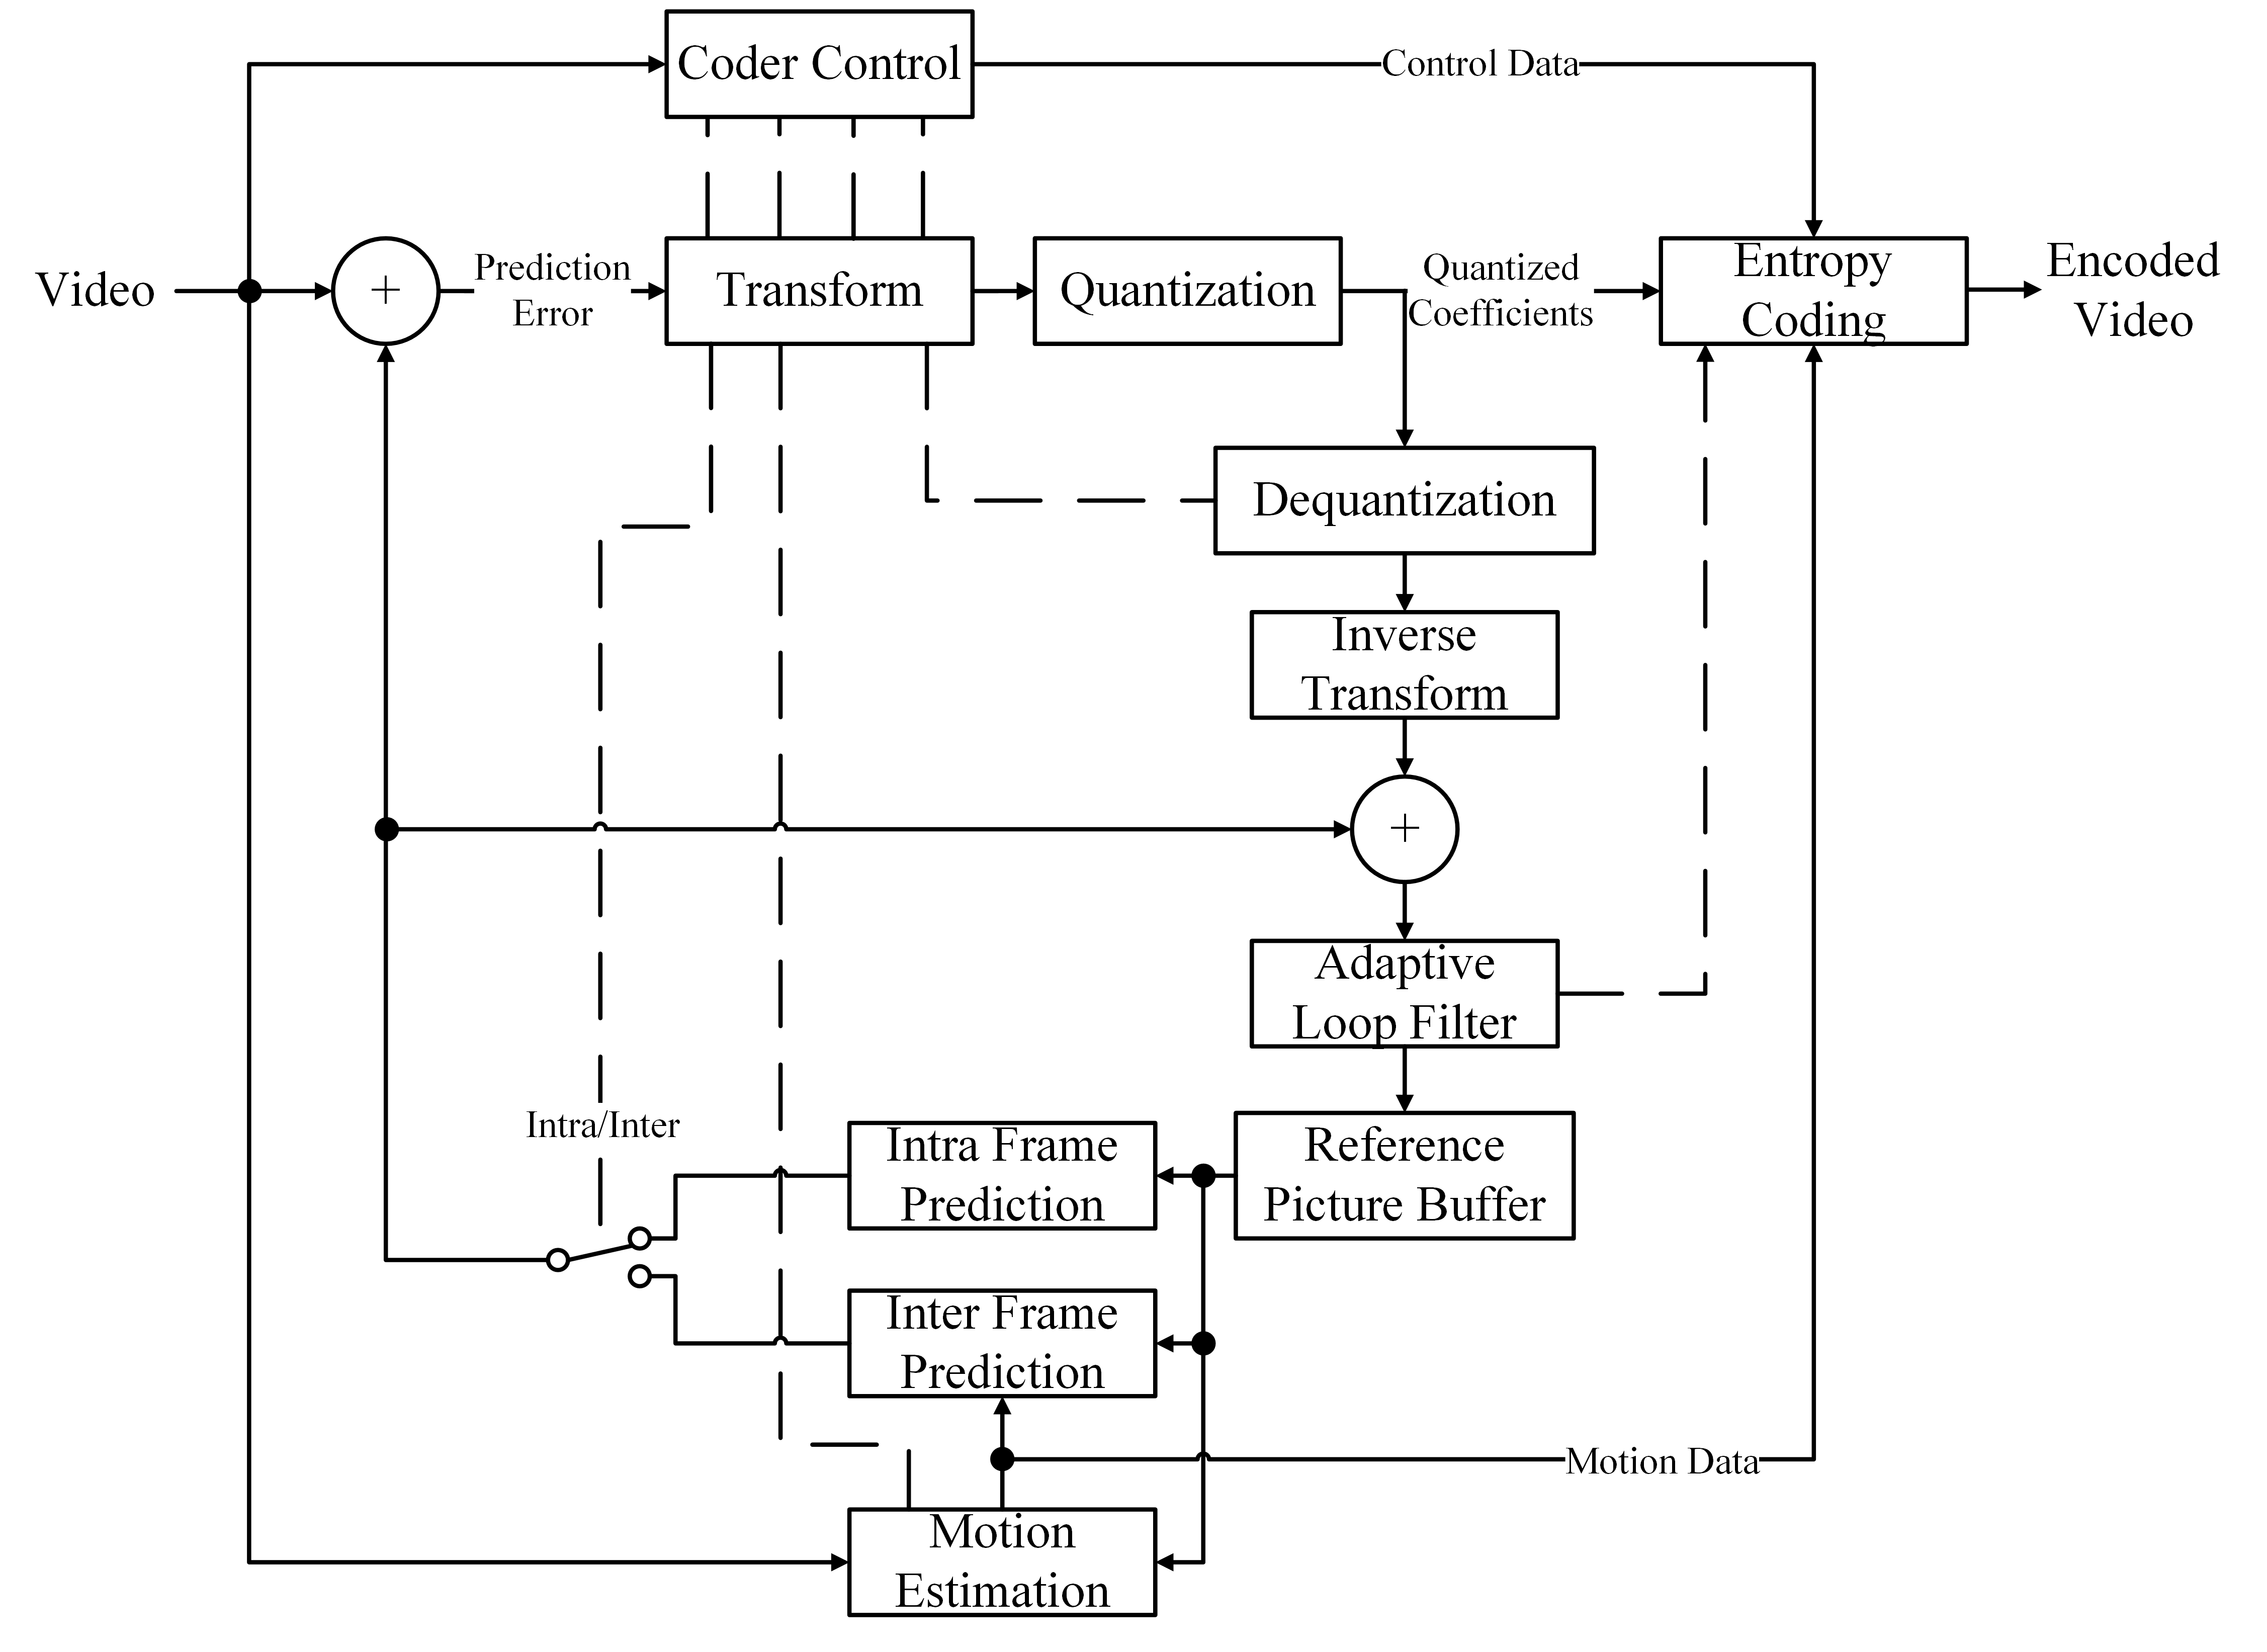
\includegraphics[width=0.95\linewidth]{assets/h265_blockdiagram.png}
        \caption{Block Diagram of High Efficiency Video Coding}
        \label{fig:hevc}
    \end{figure}

    The block diagram of \gls{hevc} shares a similar high-level structure with \gls{avc}, reflecting its hybrid coding framework based on intra-frame and inter-frame prediction, transform, quantization, and entropy coding. However, \gls{hevc} introduces several key advancements to improve compression efficiency, particularly for high-resolution content. Additionally, some blocks in \gls{hevc} feature entirely new functionalities.

    \begin{enumerate}[label=\textbf{\roman*.}]
        \item \textbf{Input Video:}  
        \gls{hevc} processes input video frames divided into luminance (Y) and chrominance (Cb, Cr) components, similar to H.264. However, HEVC replaces macroblocks with flexible Coding Tree Units (CTUs), which can be as large as 64×64 and recursively partitioned into smaller Coding Units (CUs), down to 8×8. This flexibility reduces overhead for high-resolution content.
    
        \item \textbf{Intra-/Intermode Decision:}  
        \gls{hevc} decides between intra-prediction (within a frame) and inter-prediction (between frames) based on the redundancy present. It offers 35 intra-prediction modes for luma and 6 for chroma, significantly improving texture handling compared to H.264's limited modes. Inter-prediction is enhanced with asymmetric motion partitions (AMPs) and motion merge mode.
    
        \item \textbf{Motion Estimation and Compensation:}  
        \gls{hevc} uses refined sub-pixel precision for motion estimation, improving upon H.264's quarter-pixel accuracy. Sophisticated search strategies optimize motion vectors and reduce complexity. Motion merge mode reuses parameters to compress the bitstream further, while multi-reference frame compensation improves prediction accuracy.
    
        \item \textbf{Transform and Quantization:}  
        \gls{hevc} supports larger transform block sizes (up to 32×32) compared to H.264's maximum of 8×8, enhancing compression for smooth areas. It introduces the Discrete Sine Transform (DST) for intra-predicted blocks and uses improved quantization techniques, simplifying the decoding process.
    
        \item \textbf{Entropy Coding:}  
        \gls{hevc} exclusively employs Context-Adaptive Binary Arithmetic Coding (CABAC), optimizing it for larger block sizes and parallel processing, unlike H.264, which also used the less efficient Context-Adaptive Variable Length Coding (CAVLC).
    
        \item \textbf{Deblocking Filter:}  
        \gls{hevc} improves deblocking decisions by considering multiple block boundary types (e.g., CUs, PUs, TUs). This provides better artifact suppression, especially for high-resolution content.
    
        \item \textbf{Adaptive Loop Filtering (ALF):}  
        \gls{hevc} applies adaptive filters optimized for each frame's content, reducing distortions introduced during encoding. This ensures better visual quality by minimizing blocking and blurring artifacts.
    
        \item \textbf{Reference Picture Buffer:}  
        \gls{hevc} stores reference frames in an optimized buffer, supporting larger coding tree units and parallel processing methods like wavefront parallel processing.
    
        \item \textbf{Coder Control:}  
        \gls{hevc} integrates advanced coder control to manage partitioning, mode selection, and bit allocation. It supports parallel encoding strategies to maximize multi-core processor efficiency.
    \end{enumerate}


\pagebreak

